\chapter{Экспериментальное исследование оптических частотных гребенок в кристаллических микрорезонаторах} \label{chapt3}

\section{Изготовление кристаллических микрорезонаторов методом алмазного точения и полировки}

В литературе были продемонстрированы следующие способы изготовления микрорезонаторов:

\begin{itemize}
  \item Плавление в пламени водородной горелки для микросфер из плавленого кварца.
  \item Выжигание мощным лазером $CO_2$ вращающейся заготовки.
  \item Механическое точение резонаторов.
  \item Различные литографические методы для изготовление интегральных микрорезонаторов.
\end{itemize}

В данной работе для изготовления всех микрорезонаторов из кристаллических материалов изучался и использовался метод алмазного точения с последующей полировкой алмазными суспензиями.

Чертеж микрорезонатора на подставке дан на рис. \ref{cavity_scheme_big}. Основные характеристики цилиндрического микрорезонатора - диаметр, толщина и радиус закругления боковой поверхности, где сосредоточено электрическое поле моды шепчущей галереи. Геометрия изготовленных образцов менялась в следующих пределах: диаметр 150 мкм – 12 мм (ОСД $FSR= \frac{c}{2\pi Rn}$, где $R$ – радиус резонатора), толщина 20 мкм – 6 мм и радиус закругления от 35 мкм до $R/2$.

\begin{figure}[ht]
    \centering
  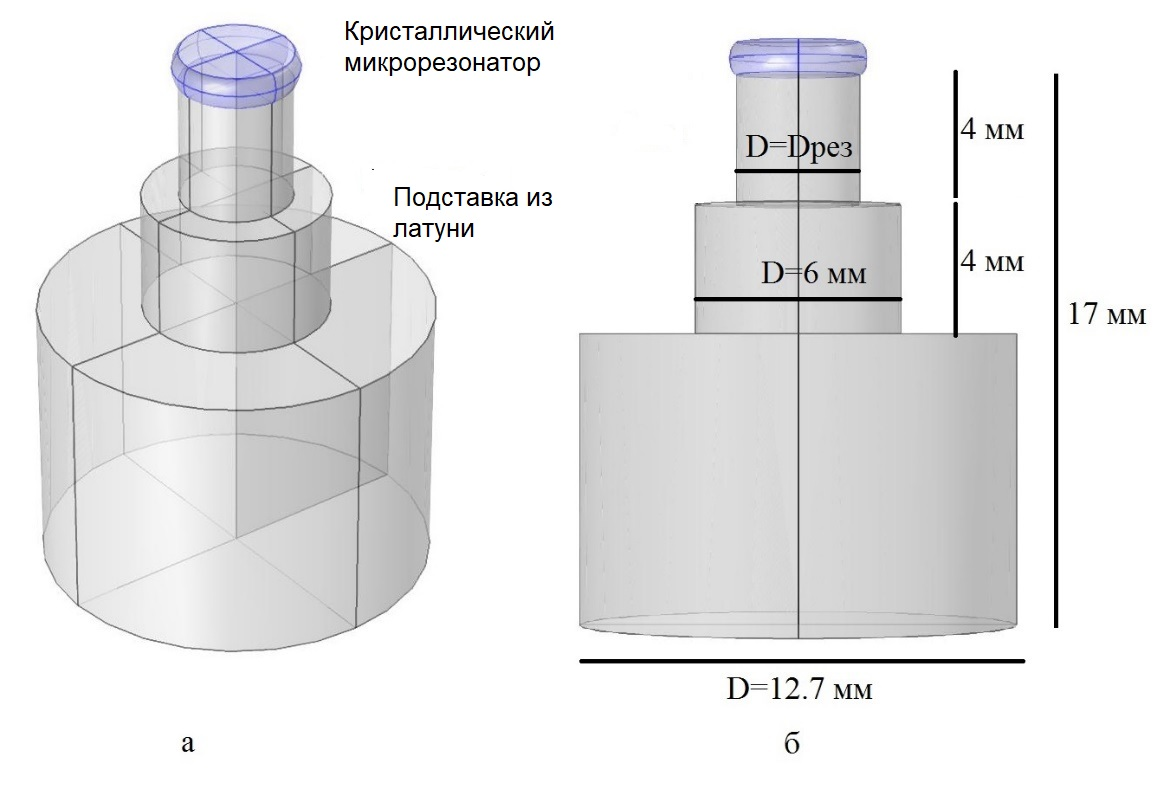
\includegraphics[width=0.5\linewidth]{cavity_scheme_big}
  \caption{Схема кристаллического микрорезонатора на подставке.}
  \label{cavity_scheme_big}
\end{figure}

Для изготовления микрорезонаторов использовались кристаллические пластины фторида магния ($MgF_2$), фторида кальция ($CaF_2$), фторида бария ($BaF_2$), фторида стронция ($SrF_2$), фторида лития ($LiF$), ниобата лития ($LiNbO_3$), танталата лития ($LiTaO_3$), кремния ($Si$), кристаллического кварца ($SiO_2$), тербий галлиевого граната (TGG) и нескольких активных кристаллов ($YLiF_4:Yb, YLiF_4:Tm, YLiF_4:Er$).

Микрорезонаторы из перечисленных материалов не могут быть изготовлены путем обжига пламенем или мощным $CO_2$ лазером. Также не найдены литографические способы (CMOS совместимые или иные, кроме кремния и ниобата лития) изготовления с необходимым качеством поверхности. Поэтому в работе использовалась механическая обработка кристаллов: точение резцыми на прецизионном токарном станке и последующая полировка алмазными суспензиями.

Для изготовления микрорезонаторов используется следующая последовательность действий:

\begin{itemize}
  \item Центрирование и наклеивание заготовки на подставку с помощью клея.
  \item Ручное стачивание заготовки до цилиндрической формы с помощью шкурок.
  \item Вытачивание цилиндра заданного диаметра алмазным резцом (возможно изношенным резцом) на прецизионном токарном станке.
  \item Вытачивание на цилиндре микрорезонатора с заданной геометрией с помощью чистового (нового) алмазного резца.
  \item Очистка микрорезонатора с помощью полимерной салфетки с изопропанолом, метанолом или ацетоном высокой чистоты.
  \item Проверка качества получившейся поверхности в микроскоп или оптический профилометр.
\end{itemize}

Хотя метод алмазного точения (SPDT, single point diamond turning) давно изучался в литературе и успешно используется в некотором количестве приложений, строгой теории для оптимального процесса точения нет. Для достижения наилучшего качества поверхности кристаллов в литературе, как правило, указывается на необходимость уменьшения всех параметров: глубины захода резки, скорости вращения шпинделя и скорости движения резца. В процессе данной работы были экспериментально найдены оптимальные параметры для точения без охлаждающей жидкости.

Для точения использовался прецизионный станок с численным программном управлением, модель DAC ALM Lathe (рис. \ref{lathe}), который коммерчески используется для точения из пластика контактных линз для глаз. Станок имеет прецизионный шпиндель и подвижные оси X,Y на воздушных подшипниках. Точность движения подачи специфицирована на уровне $10$ нм. Станок управляется с помощью скриптов, написанных на проприетарном языке DSL. Станок оборудован высокоточным датчиком касания, который калибрует расстояние по оси Y до момента касания заготовки в шпинделе. Также доступен датчик высоты, с точностью измерения до 100 нм. Станок оборудован осциллирующим резцом, расположенным под углом около 45 градусов к поверхности точения, который синхронизируется с вращением шпинделя, и позволяет точить асферические поверхности (однако не позволяет делать этого на образующей цилиндра).

\begin{figure}[ht]
  \begin{minipage}[ht]{0.49\linewidth}\centering
    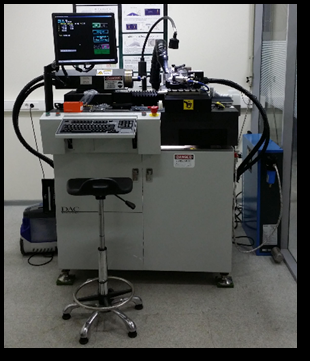
\includegraphics[width=1\linewidth]{lathe}
  \end{minipage}
  \hfill
  \begin{minipage}[ht]{0.49\linewidth}\centering
    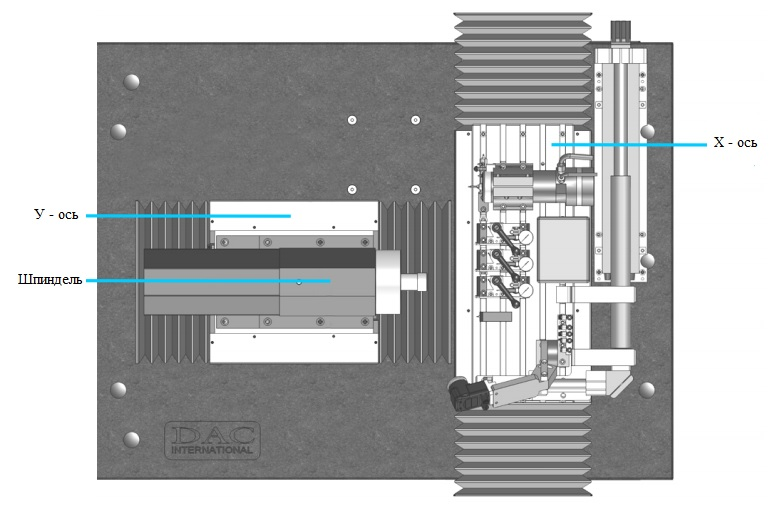
\includegraphics[width=1\linewidth]{lathe_top_view}
  \end{minipage}
  \caption{Фото используемого станка для алмазного точения DAC ALM.}
  \label{lathe}
\end{figure}

Для точения использовались поликристаллические алмазные резцы производства KY Diamonds (рис. \ref{diamond_tools}): 1) с радиусом кривизны около 500 мкм, рабочей дугой окружности в 120 градусов, с 0 или -25 углом наклона рабочего края, конический задний угол резца 10 градусов; 2) с радиусом кривизны 100-200 мкм, рабочей дугой окружности в 60 градусов, с -25 углом наклона рабочего края, цилиндрический задний угол резца 8 градусов; 3) острый резец невыдержанным радиусом кривизны 4 мкм, 0 угол наклона рабочего края. Радиусом кривизны острия алмаза (рабочей кромки) составляет 30 нм. Алмазные резцы располагались в держателях перпендикулярно или под углом около 80 градусов к оси вращения шпинделя.

\begin{figure}[ht]
  \begin{minipage}[ht]{0.24\linewidth}\centering
    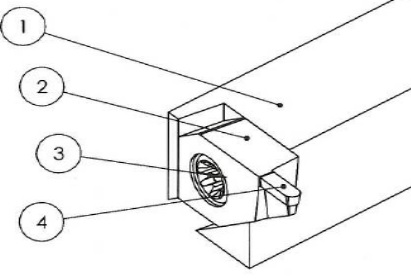
\includegraphics[width=1\linewidth]{tool1}
  \end{minipage}
  \hfill
  \begin{minipage}[ht]{0.24\linewidth}\centering
    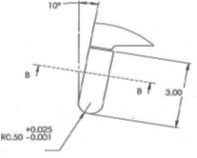
\includegraphics[width=1\linewidth]{tool2}
  \end{minipage}
  \hfill
  \begin{minipage}[ht]{0.24\linewidth}\centering
    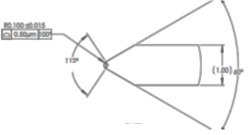
\includegraphics[width=1\linewidth]{tool3}
  \end{minipage}
  \hfill
  \begin{minipage}[ht]{0.24\linewidth}\centering
    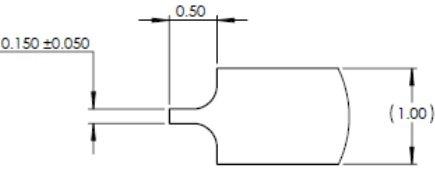
\includegraphics[width=1\linewidth]{tool4}
  \end{minipage}
  \caption{Фотографии используемых алмазных резцов с разным радиусом кривизны и углом наклона рабочей грани. Радиус кривизны рабочей кромки составляет 30 нм.}
  \label{diamond_tools}
\end{figure}

%\begin{itemize}
%    \item В цангу вставляется заготовка (пластиковый цилиндр) диаметром 12.7 мм. Шпиндель подводится к калибруемому резцу. Выставляется на глаз отступ по оси Y до момента появления стружки (касания алмазного резца).
%    \item Запускается программа, которая датчиком измеряет расстояние между фронтальной рабочей поверхностью до и после снятия слоя заданной толщины (например, 50 мкм). Точно зная это расстояние, окончательно калибруется зазор между датчиком расстояния LVDT и рабочей точкой резца.
%    \item Запускается программа, наносящая штрих глубиной 1 мкм от края заготовки до ее центра (без вращения шпинделя). В оптический микроскоп (увеличение 40x) измеряется расстояние от центра заготовки до штриха (рис. \ref{tool_calibration}). Для правильной калибровки рабочая кромка резца изначально должна быть немного ниже центра. Используя датчик высоты, подстраивается высота калибруемого резца. Процедура повторяется до тех пор, пока штрих не будет проходить строго через центр заготовки.
%    \item Проводится автоматическая калибровка расстояния по оси Х от рабочей точки алмазного резца до центра заготовки путем вытачивания трех концентрических окружностей: две при вращении шпинделя по часовой стрелке с одной стороны от центра, третья при вращении шпинделя в обратную сторону с другой стороны от центра. Далее измеряется получившееся расстояние между этими окружностями (с помощью датчика LVDT) и корректируется величина отступа между рабочей точкой резца и центром заготовки по оси X.
%    \item В конце проводится калибровка расстояния по оси X до рабочей точки резца при точении цилиндра. Важно отметить, что точение фронтальной поверхности заготовки (перпендикулярно оси вращения шпинделя) и точение боковой поверхности цилиндра (параллельно оси вращения) осуществляется разными точками. Калибровка проводится путем вытачивания цилиндра заданного диаметра с последующим измерением получившегося диаметра с помощью микрометра. При необходимости расстояние по оси Х корректируется, и калибровка повторяется. Стоит подчеркнуть, что эта калибровка наименее точная из всех, т.к. погрешность микрометра при измерении диаметра цилиндра из мягкого пластика может составлять 5-10 мкм.
%\end{itemize}


%\begin{figure}[ht]
%    \centering
%  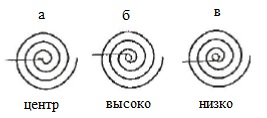
\includegraphics[width=0.5\linewidth]{tool_calibration}
%  \caption{Результат калибровки высоты резца (правильная калибровка, резец высоко, резец низко).}
%  \label{tool_calibration}
%\end{figure}

Калибровка резцов проводилась после каждой смены алмаза, калибровка Калибровка резцов проводилась сначала по оси У, что определяет точность точения толщины и расположения выступа по высоте (отступ от края). Далее проводилась калибровка резца по высоте с помощью датчика высоты. Это важный этап, т.к. угол наклона рабочей плоскости резца существенно влияет на режим точения. На финальном этапе калибруется расстояние по оси X до рабочей точки резца (калибровка диаметра резонатора). Точение фронтальной поверхности заготовки (перпендикулярно оси вращения шпинделя) и точение образующей цилиндра (параллельно оси вращения) осуществляется разными точками алмаза. Калибровка проводилась путем точения пластиковых цилиндров заданного диаметра и его измерением с помощью микрометра. Калибровка диаметра (оси Х) наименее точная, т.к. погрешность измерения диаметра цилиндра из мягкого пластика с помощью обычного микрометра может составлять 5-10 мкм.

Далее кристаллические заготовки наклеиваются на подставку из латуни. В работе использовались клеи от производителя Norland (марки NOA 60, 61, 65, 68), которые быстро отвердевают при облучении УФ лампой. Лучший результат был достигнут с NOA 61, 65. Время полного отвердевания под ультрафиолетовой лампой (длина волны 365 нм и мощность 27 Вт/см$^2$) составляло 15 мин. В начале разработки методики изготовления использовались эпоксидная смола, этилцианакрилат, и двухкомпонентные термоклеи AremCo, которые также давали хороший результат, и позволяли наклеивать непрозрачные в УФ диапазоне материалы или материалы с металлическим напылением. Минимальный диаметр микрорезонатора, при котором он не отклеивался при точении, составил около 800 мкм. Для меньших диаметров резонатора требуется сохранять кристаллическую ножку большего диаметра, вытачивая сам резонатор на кончике заготовки. Были испытаны двухкомпонентные клеи производителя AremCo, отвердевающие за сутки при температуре 94 С, и выдерживающие температуру нагревания в 400 С.

Были написаны программы на языке DSL для точения из кристаллических заготовок микрорезонаторов с боковой поверхностью (образующей) с заданным радиусом кривизны или с микровыступом в форме трапеции или прямоугольника. Параметры возможной геометрии микрорезонатора ограничены, как правило, геометрией (углом и радиусом кривизны) используемого алмазного резца.


\begin{figure}[ht]
  \begin{minipage}[ht]{0.49\linewidth}\centering
    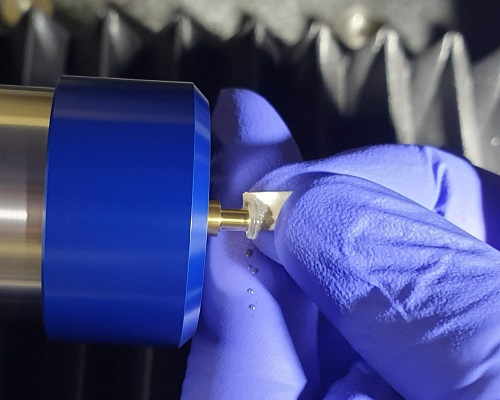
\includegraphics[width=1\linewidth]{cavity_fab_polishing_new}
  \end{minipage}
  \hfill
  \begin{minipage}[ht]{0.49\linewidth}\centering
    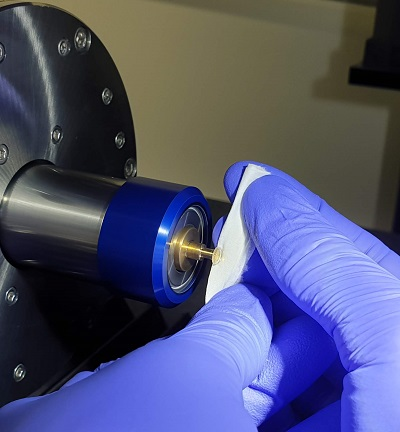
\includegraphics[width=1\linewidth]{cavity_fab_cleaning}
  \end{minipage}
  \caption{Фото процесса ручной полировки алмазной суспензией (слева). Очистка резонатора от пыли или остатков суспензий проводилась с использованием метилового спирта или ацетона и салфеток Kimwipes (справа).}
  \label{cavity_fab}
\end{figure}

\begin{figure}[ht]
  \begin{minipage}[ht]{0.49\linewidth}\centering
    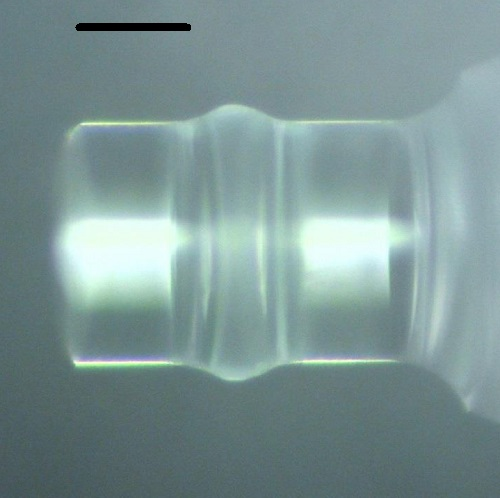
\includegraphics[width=1\linewidth]{cavity_fab_small}
  \end{minipage}
  \hfill
  \begin{minipage}[ht]{0.25\linewidth}\centering
    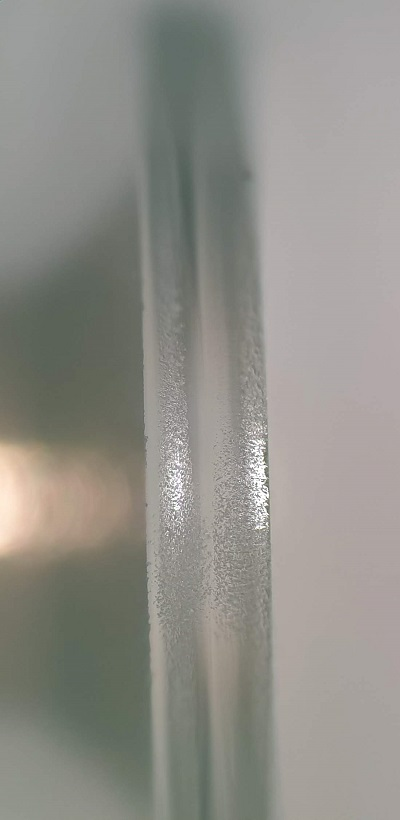
\includegraphics[width=1\linewidth]{LN_unpolished}
  \end{minipage}
  \caption{Слева: Фото микрорезонатора из $MgF_2$ радиусом 125 мкм, выточенный на станке DAC ALM c ЧПУ. Справа: резонатор из $LiNbO_3$ радиусом около 2 мм и радиусом кривизны боковой грани 520 мкм, до полировки.}
  \label{cavity_small}
\end{figure}


%\begin{figure}[ht]
%\centering
%  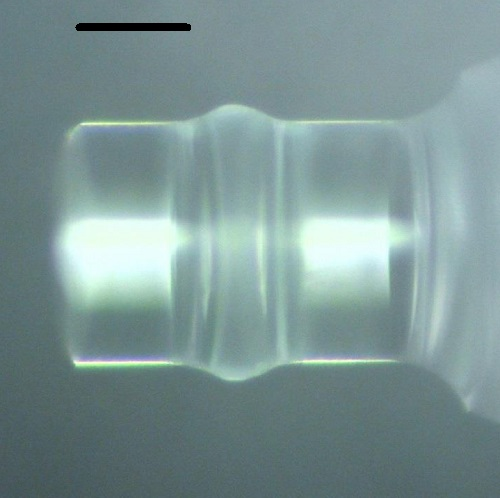
\includegraphics[width=0.5\linewidth]{cavity_fab_small}
%  \caption{Микрорезонатор ММШГ ($MgF_2$) диаметром 250 мкм и радиусом кривизны боковой поверхности 50 мкм, выточенный с помощью программы DAC DSL.}
%  \label{cavity_small}
%\end{figure}

Алгоритм и параметры работы программы для точения:
\begin{itemize}
  \item Задаются параметры программы (схематично даны на рис. \ref{cavity_scheme})
  \begin{enumerate}
    \item диаметр кристаллический заготовки (\texttt{blank\_diameter}),
    \item диаметр резонатора (\texttt{diameter}),
    \item отступ от верхней поверхности (\texttt{front\_margin})
    \item длина хорды (\texttt{chord}), на которой вытачивается выступ резонатора с радиусом кривизны (\texttt{curvature\_radius})
    \item толщина микрорезонатора (\texttt{blank\_thickness})
    \item скорость вращения шпинделя (\texttt{rpm})
    \item скорость движения резца при грубом точении цилиндра (\texttt{cylinder\_fr}) и финального чистового прохода (\texttt{fr})
    \item глубина захода резки при грубом точении цилиндра (\texttt{cylinder\_step}) и финального чистового прохода (\texttt{step\_amount\_to\_remove}).
  \end{enumerate}
  \item Грубым (изношенным) резцом обрабатывается цилиндр до заданного диаметра путем удаления слоев глубиной \texttt{cylinder\_step} со скоростью \texttt{cylinder\_fr}
  \item Чистовым (новым) резцом последовательно удаляется материал слоями глубиной \texttt{step\_amount\_to\_remove} с выступом сфероидальной формы, отступом от верхнего края (\texttt{front\_margin}) и радиусом кривизны (\texttt{curvature\_radius}) со скоростью движения резца \texttt{fr}.
\end{itemize}

\begin{figure}[ht]
\centering
  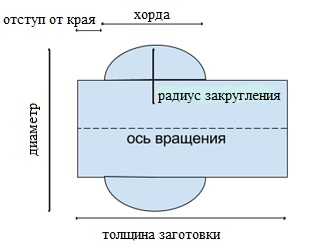
\includegraphics[width=0.5\linewidth]{cavity_scheme}
  \caption{Рисунок микрорезонатора с обозначением параметров для программы алмазного точения на языке DAC DSL.}
  \label{cavity_scheme}
\end{figure}

Ключевыми параметрами, определяющими качество поверхности изготавливаемых резонаторов, являются скорость вращения шпинделя (\texttt{rpm}), линейная скорость движения резца (\texttt{feed rate}) и глубина захода резки (\texttt{depth of cut}). Опытным путем были определены оптимальные параметры для точения кристаллов $MgF_2$:

\begin{itemize}
    \item \texttt{rpm}=300-1000, т.ч. линейная скорость точения ($rpm\times 2\pi r$) была минимальной;
    \item \texttt{feed\_rate}=2-5 мкм/оборот для грубой обработки цилиндра и <1 мкм/оборот для финального чистового прохода;
    \item \texttt{depth\_of\_cut}=2-4 мкм для грубой обработки и 0.05-1 мкм для финального прохода.
\end{itemize}

Для уменьшения износа резца и достижения пластичного режима точения твердых кристаллов использовалось охлаждение во время точения. Для этого на алмазный резец и микрорезонатор распылялась охлаждающая жидкость, которая затем уходила в воздухозаборник пылесоса вместе с кристаллическими стружками (характерным размером в сотни нм). В качестве охлаждающей жидкости использовался либо изопропиловый спирт, либо деароматизированный бензин от Exxsol. Важно, чтобы охлаждающая жидкость быстро улетучивалась и попадала внутрь шпинделя или линейных подвижных подач на воздушных подшипниках. Однако из-за длительности процесса точения одного резонатора и, соответственно, большого расхода жидкости, как правило, охлаждение не использовалось. При этом алмаз изнашивался быстрее (около 100 м точения до износа острой кромки резца). Без полировки непосредственно после точения в резонаторах из $MgF_2$ достигается добротность порядка $5\times10^5$ на 1550 нм.

После точения осуществлялась очистка резонатора от кристаллической стружки с помощью полимерных салфеток с ацетоном или метанолом. Повышение добротности резонатора достигается благодаря последовательной ручной полировкой с помощью алмазных суспензий с зерном 1, 0.5, 0.1 мкм по 10 мин каждой. Для микровыступов в форме трапеции использовалось только зерно 0.1 мкм. Использовались алмазные суспензии производства Microdiamant OPW-20, концентрация алмазных зерен 15 карат/литр, вязкость 325 cP. Суспензии наносились на специальный текстиль производства AlliedHighTech, который при ручной полировке позволял эффективнее удалять материал при более плотном касании.
 
Перед использованием резонатора всегда проводилась очистка его поверхности с помощью салфеток, смоченных в спирте. Очистка проводится чистой, плотно сложенной салфеткой с небольшим количеством спирта, однократным движением по образующей цилиндра в сторону вращения шпинделя (при rpm=400). В условиях нашей лаборатории добротность падала в течение нескольких дней в 2-3 раза из-за возможного осаждения пыли или значительного изменения влажности. После каждой очистки проводилась проверка качества поверхности в микроскоп. При увеличении в 40х возможно обнаружить шероховатости и остатки спирта или грязи порядка 1-2 мкм. Шероховатость малого размера в оптический микроскоп может быть не видна из-за дифракционного предела, на увеличении 50х глубина резкости минимальна, т.ч. наблюдается малая область сфероидальной поверхности, около 50 мкм при радиусе кривизны боковой грани 500 мкм и диаметре резонатора 4 мм. Поэтому контроль качества осуществлялся последовательным измерением добротности мод резонатора после полировки и очистки.

На рис. \ref{cavity_polished} даны фото поверхности резонатора непосредственно после точения, фрагмент с шероховатостями порядка 5 мкм и после полировки суспензиями, видно улучшение качества поверхности.

\begin{figure}[ht]
  \begin{minipage}[ht]{0.32\linewidth}\centering
    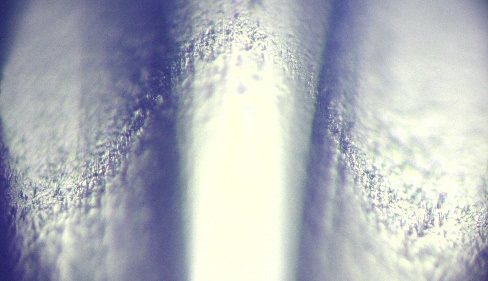
\includegraphics[width=1\linewidth]{cavity_unpolished}
  \end{minipage}
  \hfill
  \begin{minipage}[ht]{0.32\linewidth}\centering
    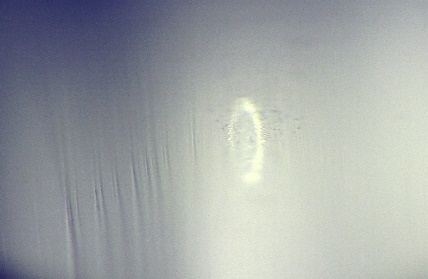
\includegraphics[width=1\linewidth]{cavity_polished_bad}
  \end{minipage}
  \hfill
  \begin{minipage}[ht]{0.32\linewidth}\centering
    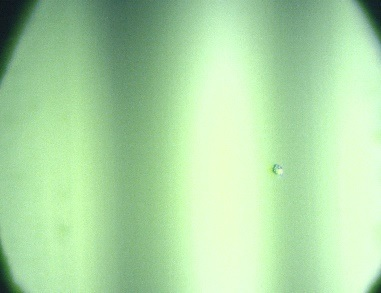
\includegraphics[width=1\linewidth]{cavity_polished_good}
  \end{minipage}
%  \caption{Фрагмент поверхности резонатора с радиусом кривизны боковой поверхности 50 мкм (ширина выступа около 70 мкм). Слева сразу после точения изношенным резцом. Посередине фрагмент со сколом размером 20 на 50 мкм. Справа - после полировки алмазными суспензиями.}
  \label{cavity_polished}
\end{figure}

Дополнительно может быть произведен контроль качества боковой поверхности с помощью оптического профилометра Zygo NewView 7300. Результат измерения приведен на рис. \ref{cavity_profilometer}, измерены шероховатости размером 0.25 мкм.

\begin{figure}[ht]
\centering
  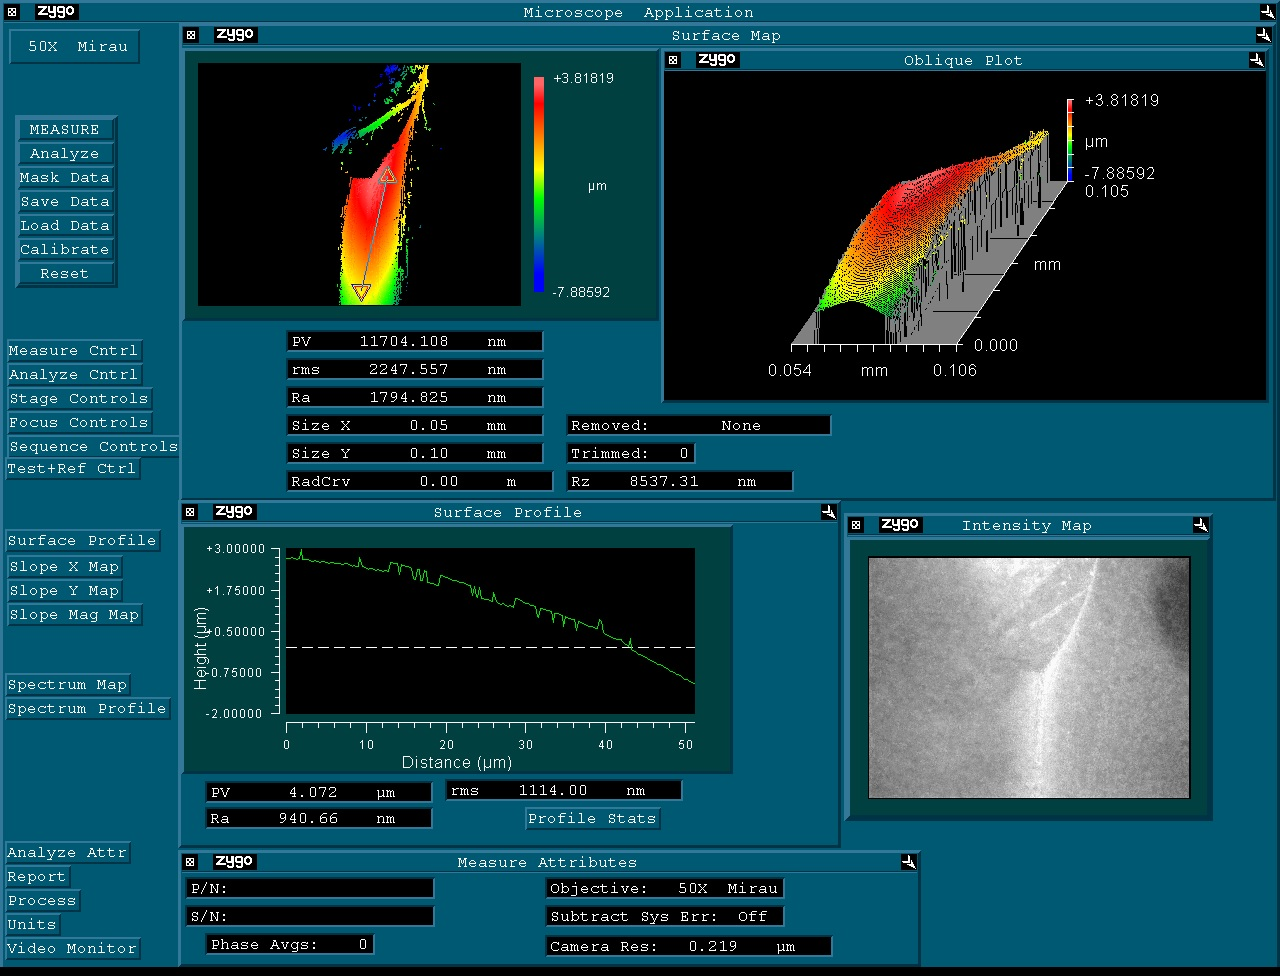
\includegraphics[width=0.5\linewidth]{cavity_profilometer}
  \caption{Измерение качества боковой поверхности с помощью оптического профилометра.}
  \label{cavity_profilometer}
\end{figure}

Достаточным условием для оценки качества поверхности является проверка добротности после полировки. К сожалению, при таком способе оценки качества поверхности можно упустить технические ошибки, возникающие при полировке, т.к. в данном случае о качестве можно судить только по косвенному признаку – добротности. Измерение добротности производилась следующими методами: калибровка частоты дается боковыми линиями фазовой модуляции сканирующего лазера, зная частоту модуляции, можно аппроксимировать лоренцевскую форму резонанса МШГ. Для измерения ширины линии резонанса меньше 500 кГц лучше использовать метод звона, при котором либо быстро выключается (с помощью акусто-оптического модулятора), либо быстро перестраивается по частоте лазер накачки, и проводится прямое измерение времени звона оптического резонатора по затухающему сигналу фотодетектора. Для измерения добротностей выше $10^9$ необходимо использовать мощность лазера меньше 500 мкВт, чтобы избежать нелинейных уширений резонанса.

В таблице \ref{table_turning_params} даны эмпирически найденные оптимальные параметры точения различных материалов.

\begin{table} [htbp]% Пример записи таблицы с номером, но без отображаемого наименования
	\centering
	\parbox{17cm}{% чтобы лучше смотрелось, подбирается самостоятельно
        %\captionsetup{format=tablenocaption}% должен стоять до самого caption
        \caption{Оптимальные параметры алмазного финального точения резонаторов из различных кристаллических материалов}%
        \label{table_turning_params}%
    	\begin{tabular}{||c|c|c|c|c||}
\hline
\multicolumn{1}{|p{2cm}|}{\centering Материал} & \multicolumn{1}{|p{2cm}|}{\centering Скорость вращения шпинделя, \\ обороты в мин} & \multicolumn{1}{|p{2cm}|}{\centering Скорость движения резца, \\ мкм/ оборот} & \multicolumn{1}{|p{2cm}|}{\centering Глубина захода резки, \\ мкм} & \multicolumn{1}{|p{2cm}|}{\centering Примечание}\\
%Материал & Скорость вращения шпинделя, обороты в мин & Скорость движения резца, мкм/оборот & Глубина захода резки, мкм & Охлаждающая жидкость\\
\hline
$MgF_2 z-cut$ & 300-1000 & 0.5-1 & 0.05-1 &  \\
\hline
$MgF_2 a-cut$ & 400-500 & 0.5-1 & 0.05-1 &  \\
\hline
$BaF_2$ & 600-1000 & 1-2 & 0.5-2 & только новым алмазом\\
\hline
$SrF_2$ & 800 & 1 & 1 & охлажд.\\
\hline
$CaF_2 z-cut$ & 400-1000 & 0.5-1 & 0.5 &  \\
\hline
$CaF_2 a-cut$ & 400 & 0.5-1 & 0.05 & охлажд.\\
\hline
$LiNbO_3$ & 900-1500 & 1-2.5 & 1-4 &  \\
\hline
$LiTaO_3$ & 900 & 1-2 & 1-2 & охлажд.\\
\hline
$Si$ & 500 & 1 & 0.5-1 &  большой износ\\
\hline
$TGG$ & 700 & 1 & 0.5-1 & охлажд.\\
\hline
$SiO_2 крист.$ & 600 & 1 & 0.5-1 & большой износ\\
\hline
$LiF$ & 900 & 1 & 1 & только новым алмазом\\
\hline
$YLiF_4:Yb$ & 400 & 2 & 1 &\\
\hline
\end{tabular}

	}
\end{table}

Изготовленные представленным методом резонаторы из $MgF_2,BaF_2,CaF_2$ были успешно испытаны с новым элементом связи - интегральной структурой, состоящей из $Si_3N_4$ волновода на чипе с вставкой из $SiO_2$ в форме мостика в воздухе \cite{Anderson:18}. Поперечное сечение $SiO_2$ составляло 2 на 5 мкм, а длина около 500 мкм. Подводя кристаллический микрорезонатор к этому мостику можно было добиться связи с различными семействами мод резонатора, была достигнута добротность более $10^8$.

\subsection{Практические замечания по изготовлению кристаллических микрорезонаторов}

Предобработка - раскол кристаллических пластин заготовок, при этом возможно образование напряжений внутри кусочков кристаллов. Мягкие материалы $BaF_2, CaF_2$ раскалываются на неконтролируемые куски при любой толщине заготовки. Распил алмазной пилой позволяет этого избежать. Однако для заготовок толщиной 100-200 мкм возможны внутренние трещины из-за неровности наклейки на подставку для распила. Необходимо использовать тонкие диски пилы с алмазным напылением. Выпиливание цилиндрических заготовок трубчатым сверлом малоэффективно, т.к. большая часть материала уходит в стружку, и из-за больших биений сверла вероятно появление больших сколов.

Дизайн подставки диктуется размером цанги станка и удобством крепления в экспериментальных установках. Материал подставки латунь выбран из-за достаточно высокой теплопроводности для улучшения активной термостабилизации. В основном кристаллические материалы для генерации оптических гребенок имели z-cut, т.ч. оптическая ось z совпадала с осью цилиндра. Отдельно были изучены кристаллы среза a-cut $MgF_2$, в котором также наблюдалась оптическая гребенка и кристалл $CaF_2$ a-cut, в котором не было областей шероховатости после точения.

Отжиг кристаллов для устранения внутренних дефектов проводился, но без прямого измерения улучшения добротности до и после, т.к. клей не позволяет нагревать до 900С наклееный на подставку резонатор, а в случае переклейки резонатора вероятность загрязнения велика, и будет требоваться новая переполировка. При попытке отжига наклеенного резонатора из $BaF_2$ при 400С в кристалле возникло большое количество внутренних трещин. Отжиг отполированного резонатора из $MgF_2$ в воздухе при 1000 С в течение 16 часов (с медленным нагревом и остыванием по 1С/мин) приводил к тому, что в приповерхностном слое толщиной около 50 мкм, кристалл становился непрозрачным (белым) и никакой добротности не наблюдалось. Для отжига требуется атмосфера из чистого азота.

Алмазное точение SPDT возможно в широком диапазоне параметров при использовании нового неизношенного резца. Качество поверхности фторида магния при этом высокое, т.ч. добротность резонатора может достигать $10^6$ (пример выступа резонатора с такой добротностью дан на рис. \ref{protrusion_unpolished}), что соответствует типичным значениям добротности в интегральных оптических резонаторах из $SiN$.

\begin{figure}[ht]
\centering
  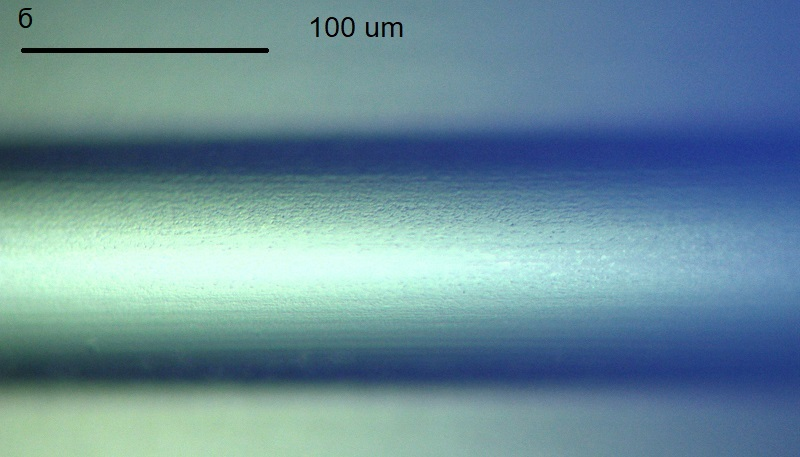
\includegraphics[width=0.5\linewidth]{protrusion_unpolished}
  \caption{Фотография поверхности резонатора из $MgF_2$ сразу после точения, в котором достигается добротность $10^6$ на 1550 нм.}
  \label{protrusion_unpolished}
\end{figure}

Основной недостаток метода алмазного точения - быстрый износ алмазного резца. На практике износ резца наступает за 100 м точения, что соответствует изготовлению 3 резонаторов. Далее качество получаемой поверхности заметно ухудшается и никакими более щадящими параметрами точения улучшить его нельзя. Изношенным резцом возможно точение твердых материалов $MgF_2$, но более мягкие $BaF_2, LiF$ могут давать сколы размерами в несколько сот микрон, недоступными для устранения \ref{cavity_damage}. Наиболее практично использовать для изготовления цилиндров заданного диаметра изношенный резец, а далее снимать финальный слой толщиной 10 мкм с помощью чистового неизношенного резца. Важно при этом регулярно проводить перекалибровку относительного положения изношенного и чистового резцов, т.к. сколы края алмаза могут достигать 10 мкм \ref{tool_damage}.

\begin{figure}[ht]
  \begin{minipage}[ht]{0.49\linewidth}\centering
    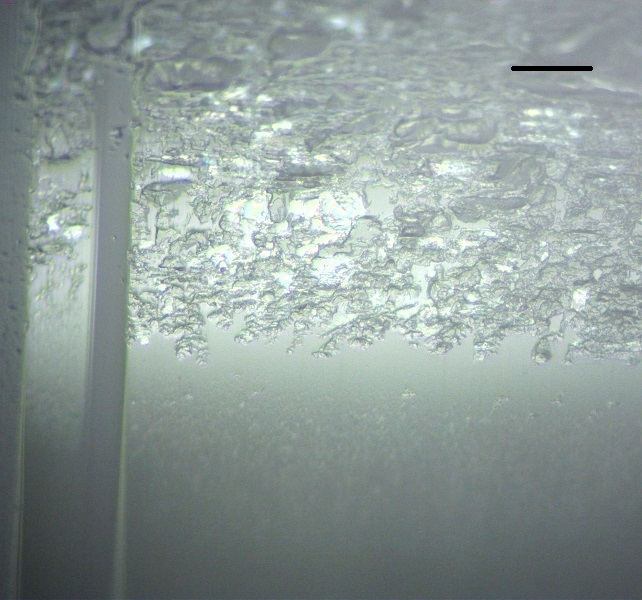
\includegraphics[width=0.6\linewidth]{cavity_damage}
  \end{minipage}
  \hfill
  \begin{minipage}[ht]{0.49\linewidth}\centering
    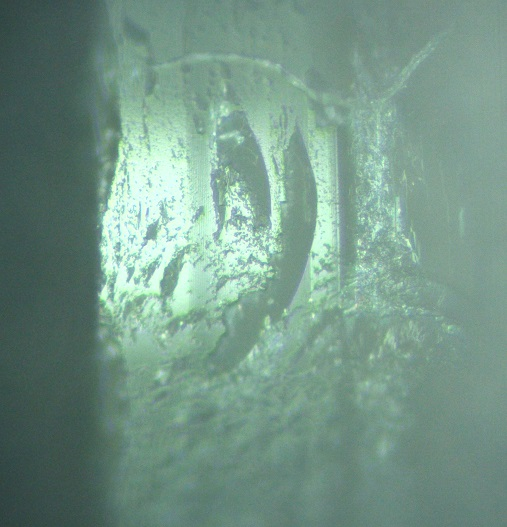
\includegraphics[width=0.6\linewidth]{cavity_damage_baf2}
  \end{minipage}
  \caption{Слева фрагмент поверхности резонатора из $MgF_2$ после точения при неоптимальных параметрах, видны секторы хорошего и плохого качества поверхности, соответствующие точению различных кристаллических срезов, такие дефекты можно убрать полировкой без сохранения геометрии резонатора. Справа фрагмент поверхности резонатора из $BaF_2$ после точения изношенным резцом, видны глубокие сколы, которые нельзя убрать полировкой.}
  \label{cavity_damage}
\end{figure}

\begin{figure}[ht]
  \begin{minipage}[ht]{0.49\linewidth}\centering
    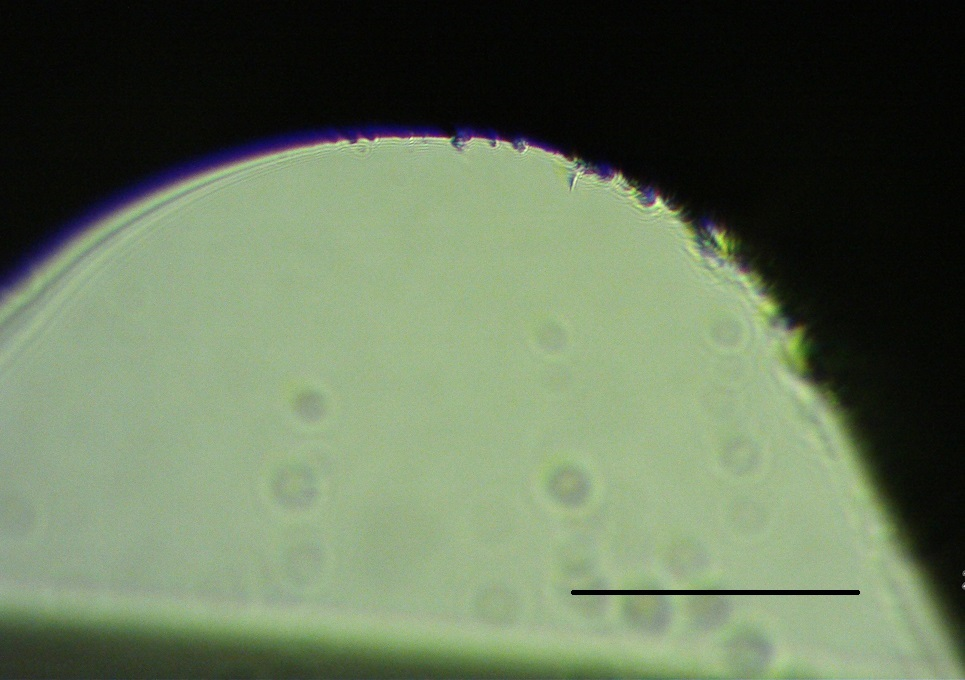
\includegraphics[width=0.7\linewidth]{tool_damage}
  \end{minipage}
  \hfill
  \begin{minipage}[ht]{0.49\linewidth}\centering
    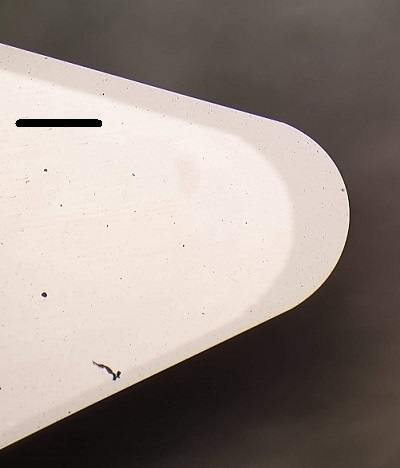
\includegraphics[width=0.6\linewidth]{fresh_tool}
  \end{minipage}
  \caption{(Слева): Рабочий край изношенного алмазного резца с радиусом кривизны 500 мкм и наклоном рабочей грани -25, видны сколы по краю характерным размером 10 мкм. При дальнейшем использовании резца возможно образование скола алмаза по прямой линии, таким резцом можно грубо вытачивать цилиндры заданного диаметра. (Справа): фотография нового резца с радиусом кривизны 200 мкм}
  \label{tool_damage}
\end{figure}


%\begin{figure}[ht]
%\centering
%  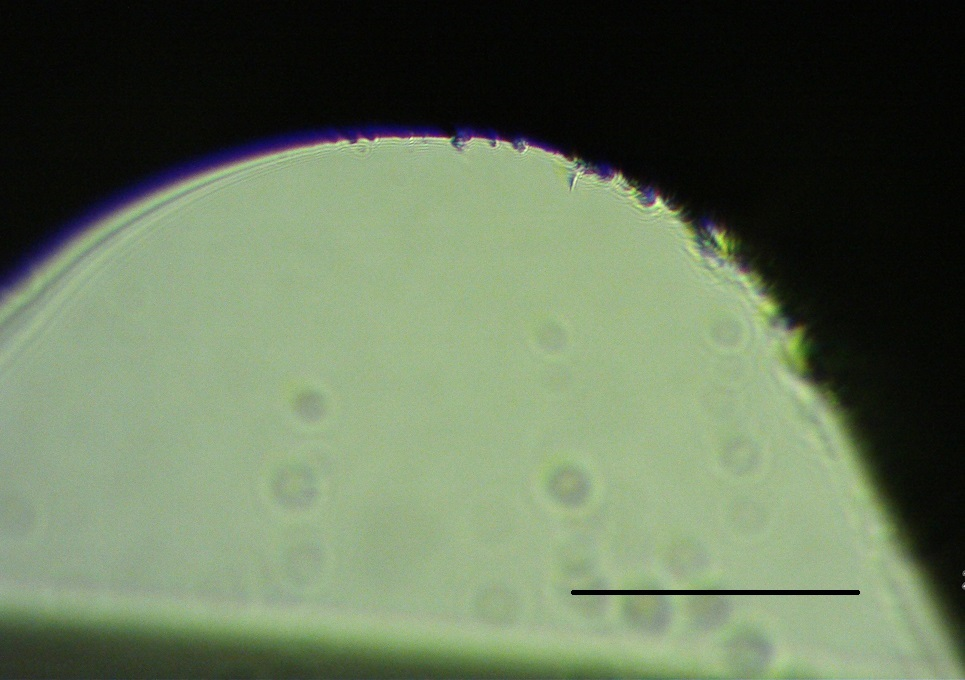
\includegraphics[width=0.3\linewidth]{tool_damage}
%  \caption{Рабочий край изношенного алмазного резца с радиусом кривизны 500 мкм и наклоном рабочей грани -25, видны сколы по краю характерным размером 10 мкм. При дальнейшем использовании резца возможно образование скола алмаза по прямой линии, таким резцом можно грубо вытачивать цилиндры заданного диаметра.}
%  \label{tool_damage}
%\end{figure}

В литературе по точению основными методами борьбы с износом являются более щадящие параметры точения (уменьшение глубины резки и действующей силы, пропорциональной скорости вращения) и использовании охлаждающей жидкости. Важно понимать, что при использовании охлаждающей жидкости меняется режим точения, и следует заново подбирать оптимальные параметры. Уменьшение же глубины резки приводит к пропорциональному росту времени точения. Охлаждающая жидкость при изготовлении большинства резонаторов из $MgF_2$ не применялась, т.к. нет удобной системы вентиляции, и ее расход велик, т.ч. бака с жидкостью может не хватать на типичное точение в 6-10 часов, также заводская жидкость содержала маслянистые фракции, которые могут повредить шпиндель на воздушных подшипниках.

Полировка при хорошей центровке микрорезонатора возможна не только последовательным уменьшением зерна суспензии, но и при грубой полировке зерном 2.5-4 мкм для удалений сколов с характерными размерами 5-15 мкм, далее зерном 0.5 мкм и сразу 0.1 мкм для финальной полировки. Стандартное правило - удаление материала в 3-4 кратном размере диаметра зерна. Таким способом повторяемо достигается добротность $5*10^8$ на длине волны $1550 нм$ в кристаллах $MgF_2$ из заготовки VUV качества материала \ref{ringdown}.

\begin{figure}[ht]
\centering
  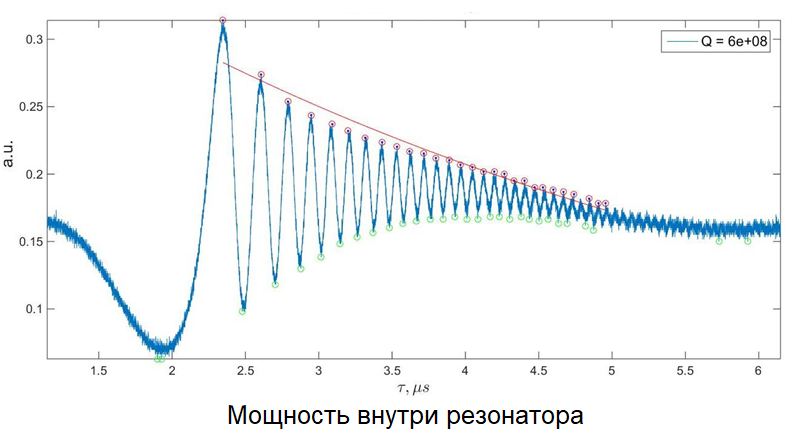
\includegraphics[width=0.5\linewidth]{ringdown1billion}
  \caption{Определение добротности резонатора из $MgF_2$ прямым измерением времени звона оптического резонатора. Соответствующее значение добротности $6*10^8$}
  \label{ringdown}
\end{figure}


Изготовление прямоугольных микровыступов даже новыми острыми резцами не удалось для диаметров резонатора больше 4 мм для $MgF_2$ и получилось для диаметров около 1 мм \ref{protrsuion_rect}. Этот резонатор далее в экспериментах не изучался.

\begin{figure}[ht]
  \begin{minipage}[ht]{0.49\linewidth}\centering
    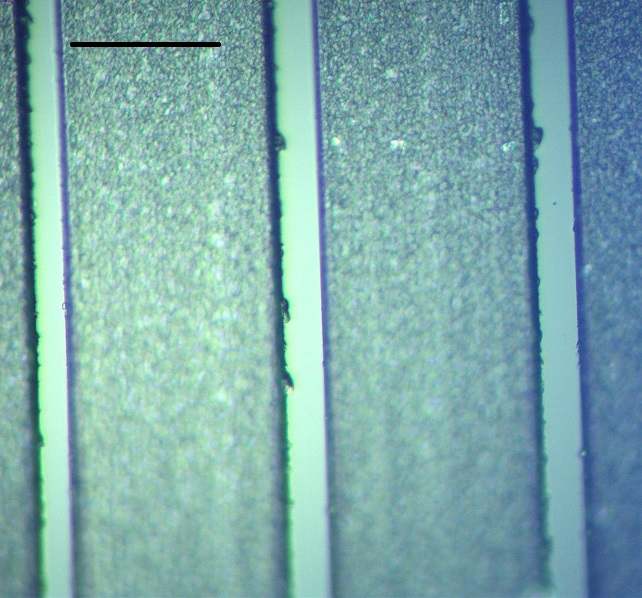
\includegraphics[width=0.6\linewidth]{protrsuion_rect}
  \end{minipage}
  \hfill
  \begin{minipage}[ht]{0.49\linewidth}\centering
    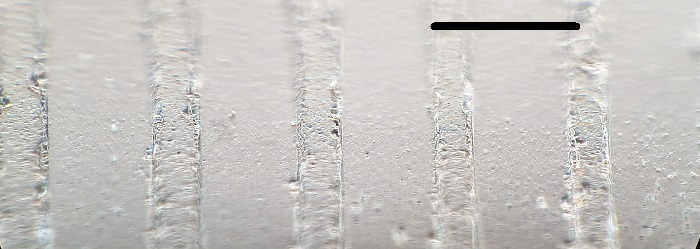
\includegraphics[width=1\linewidth]{protrsuion_rect_DF.jpg}
  \end{minipage}
  \caption{Слева: фрагмент поверхности резонатора из $MgF_2$ с прямоугольными выступами размером 5 на 20, 25 мкм для контроля ДГС резонатора. Показано качество поверхности до полировки, видны сколы по 5 мкм на выступе из-за износа острого резца. Справа: фотография выступов с другого резонатора в темном поле}
  \label{protrsuion_rect}
\end{figure}


%\begin{figure}[ht]
%\centering
%  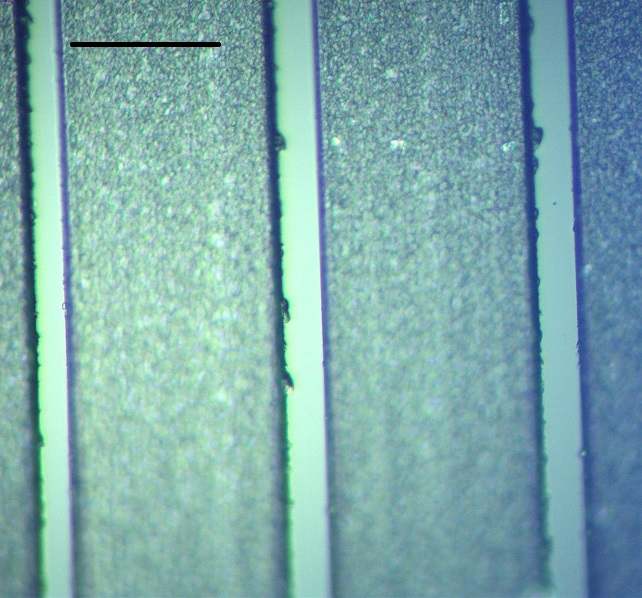
\includegraphics[width=0.5\linewidth]{protrsuion_rect}
%  \caption{Фрагмент поверхности резонатора с прямоугольными выступами размером 5 на 15, 20, 25 мкм для контроля ДГС резонатора. Показано качество поверхности до полировки, видны сколы по 5 мкм на выступе из-за износа острого резца.}
%  \label{protrsuion_rect}
%\end{figure}

\section{Экспериментальное наблюдение оптических частотных гребенок и солитонов в резонаторах из $MgF_2$}


\subsection{Экспериментальная установка и результаты генерации солитонов}

Для генерации оптических гребенок и солитонов в кристаллических микрорезонаторах использовалась следующая экспериментальная схема \ref{Setup_CoProp}. Волоконный узкополосный перестраиваемый лазер непрерывной мощности (Koheras Adjustik) подается на фазовый или амплитудный модулятор, далее сигнал усиливается эрбиевым волоконным усилителем (Koheras Boostik), спонтанные шумы усилителя подавляются узкополосным пропускающим оптическим фильтром (Dicon). Далее свет проходит через волоконный контроллер поляризации (FPC) и заводится в резонатор через элемент связи - растянутое волокно, через него же свет из резонаторы выводится. Волоконный Брэгговский фильтр (AOS) используется для подавления мощной линий накачки, далее оптический сигнал подается на оптический спектроанализатор (OSA) и быстрый фотодетектор, электрический сигнал с которого измеряется осциллографом и спектроанализатором.

Растянутое волокно изготавливалось методом травления в плавиковой кислоте: зачищенное от пластика волокно диаметром 125 мкм помещалось в 100 мкл каплю 40 процентной плавиковой кислоты на 15 мин, далее в буферный раствор 18 процентной кислоты, в котором волокно травилось около 30 мин. Контроль толщины осуществлялся по сигналу пропускания через волокно, наблюдалась характерная осцилляционная картина, травление прекращалось сразу после исчезновения осцилляций. Таким методом были получены волокна с конической перетяжкой и диаметром перетяжки от 3 до 8 мкм. Растянутые волокна выдерживали мощность до 300 мВт. Другим методом изготовления был стандартный метод растяжки волокна в пламени водородной горелки.

\begin{figure}[ht]
\centering
  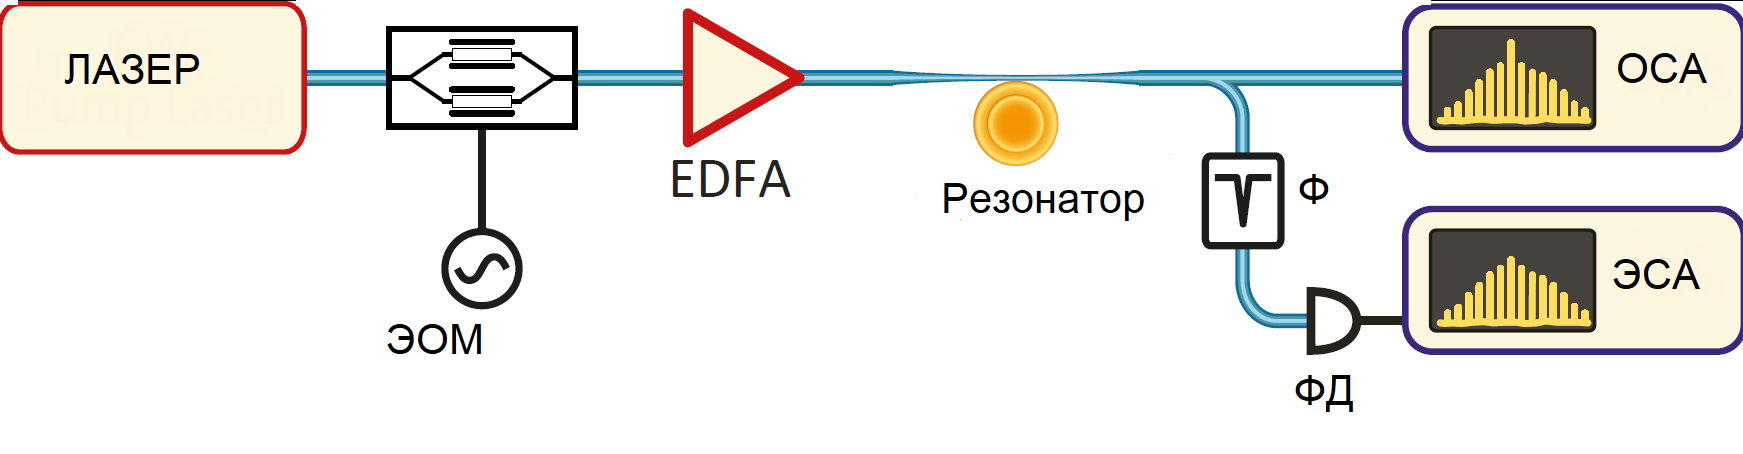
\includegraphics[width=0.4\linewidth]{Setup_CoProp}
  \caption{Cхема экспериментальной установки для генерации оптических гребенок и солитонов.}
  \label{Setup_CoProp}
\end{figure}

Для настройки на шумную гребенку \ref{step_schematics} достаточно медленно перестроить частоту лазера из области синей отстройки в красную область (верхней ветви существованяи керровских частотных гребенок). Так последовательно возбуждаются одиночные боковые линии вдали от накачки (их положение определяется дисперсией второго порядка), далее благодаря каскадному четырехволновому взаимодействию, возбуждаются все линии на расстоянии 1 ОСД и гребенка полностью заполняется. Пример генерации шумных оптических гребенок и широкого сигнала биений на частоте ОСД дан на рис. \ref{wide_comb_93GHz,noisy12}.

\begin{figure}[ht]
\centering
  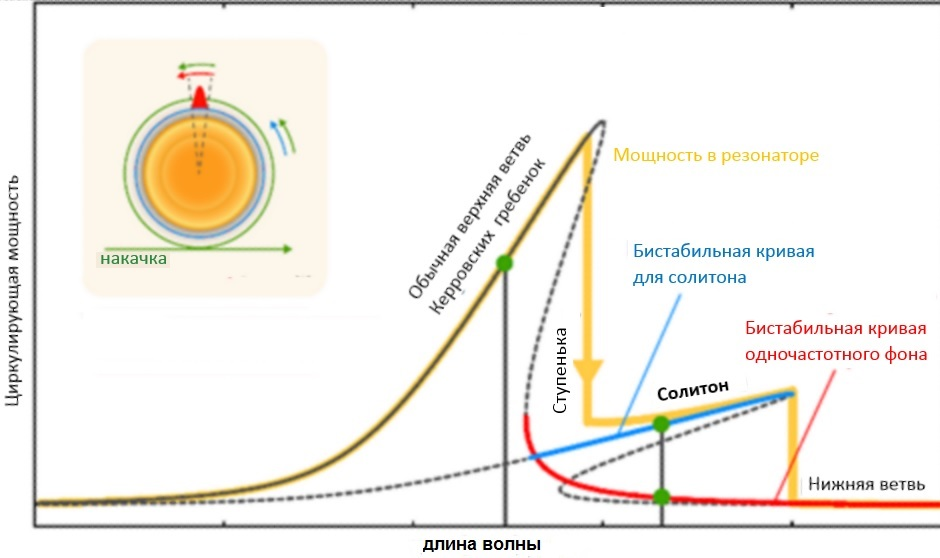
\includegraphics[width=0.6\linewidth]{step_schematics}
  \caption{Cхематичное изображение нелинейного резонанса с солитонной ступенькой и бистабильная кривая}
  \label{step_schematics}
\end{figure}

\begin{figure}[ht]
\centering
  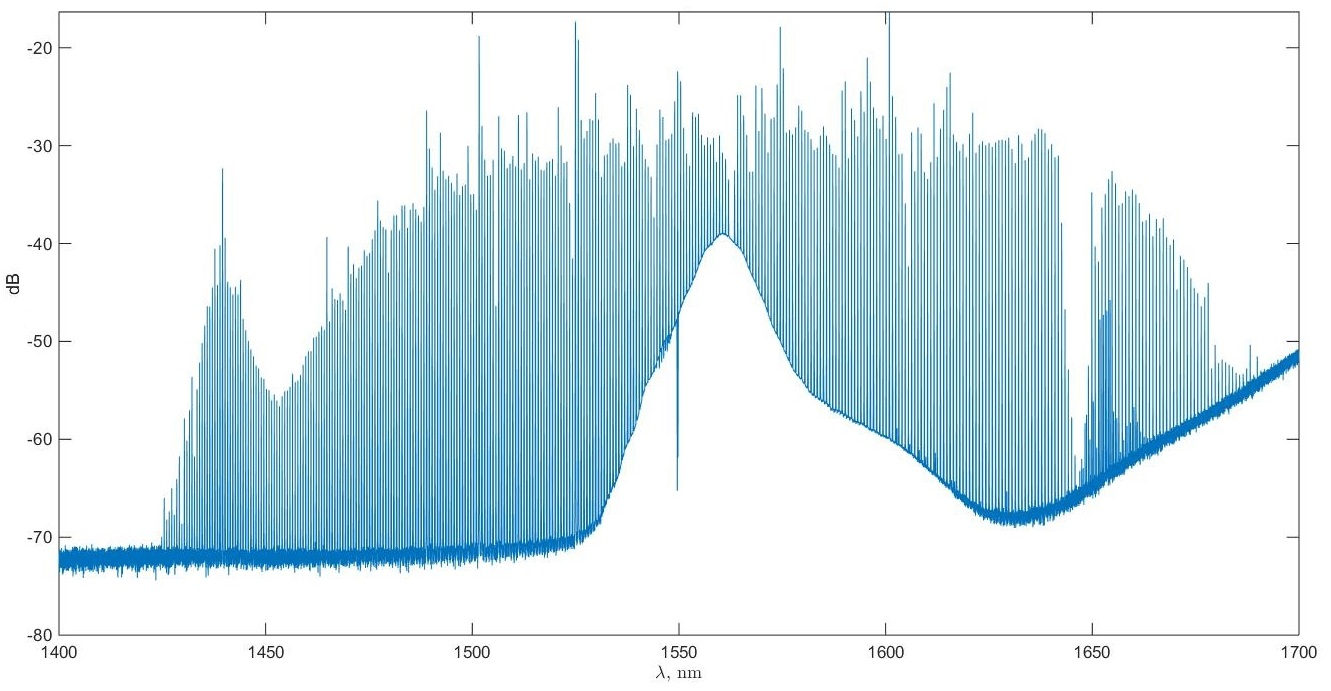
\includegraphics[width=0.5\linewidth]{wide_comb_93GHz}
  \caption{Оптический спектр широкой оптической гребенки в шумном режиме с ОСД около 93 ГГц, полученный в резонаторе диаметром 0.75 мм и радиусом кривизны 150 мкм. Видно излучение дисперсионной волны на длине волны 1440 нм.}
  \label{wide_comb_93GHz}
\end{figure}

\begin{figure}[ht]
  \begin{minipage}[ht]{0.49\linewidth}\centering
    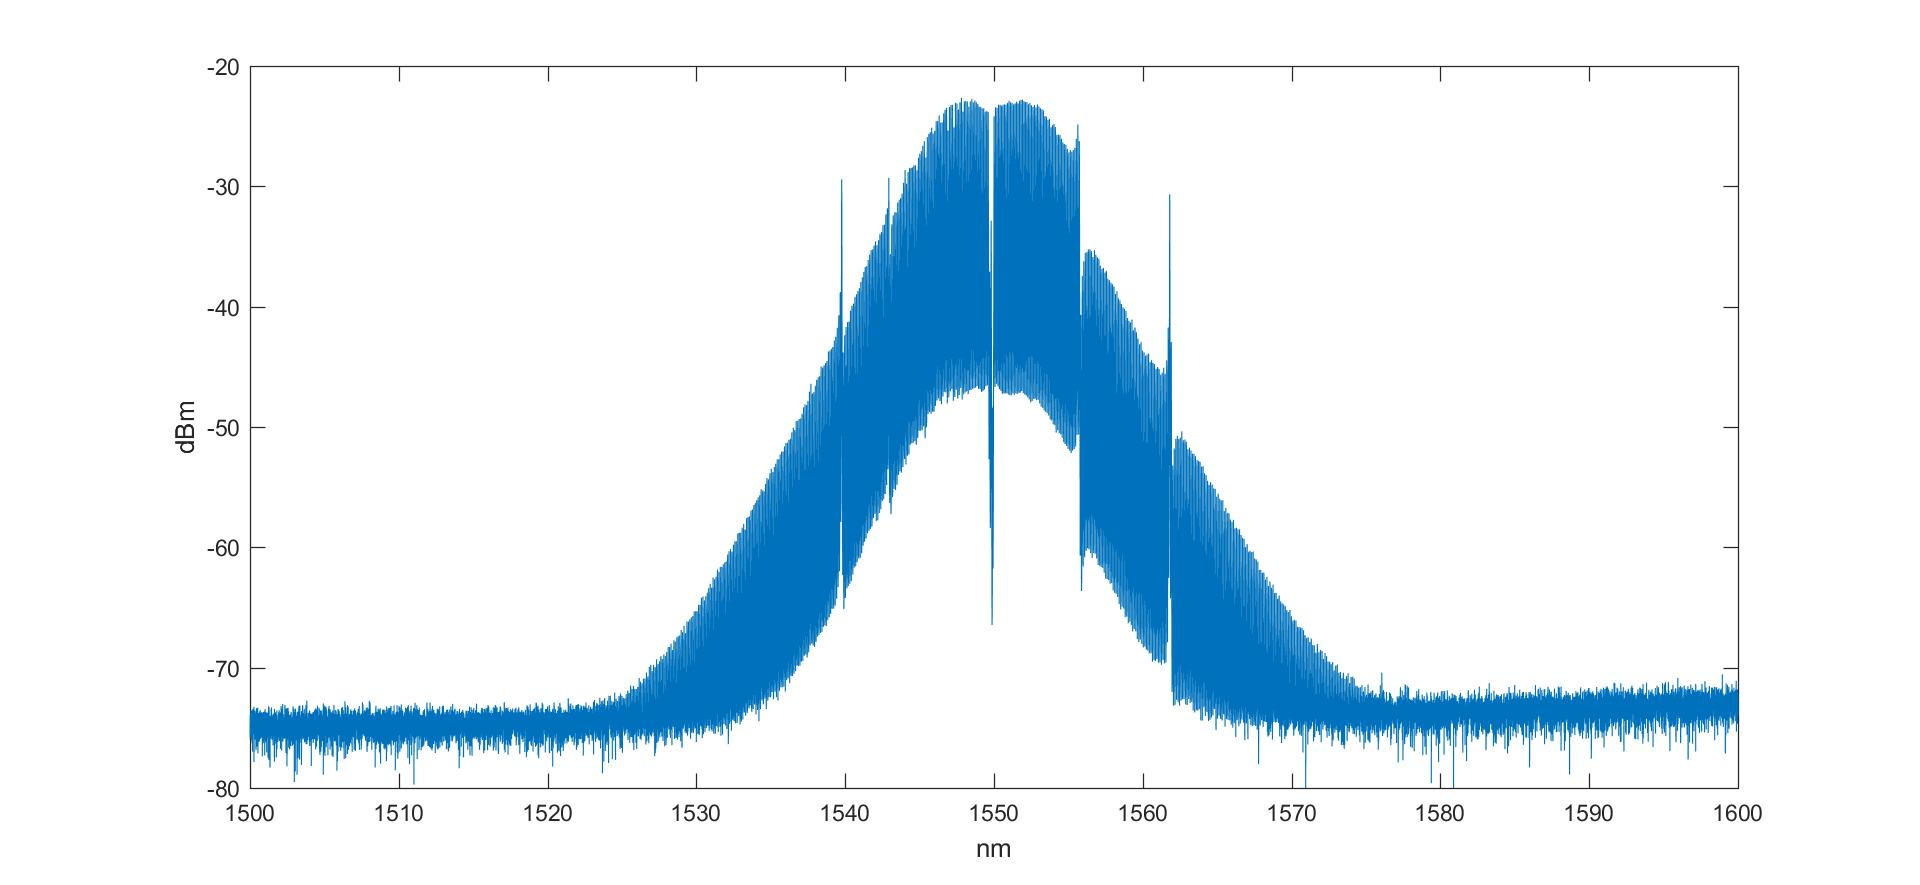
\includegraphics[width=1\linewidth]{noisy12}
  \end{minipage}
  \hfill
  \begin{minipage}[ht]{0.49\linewidth}\centering
    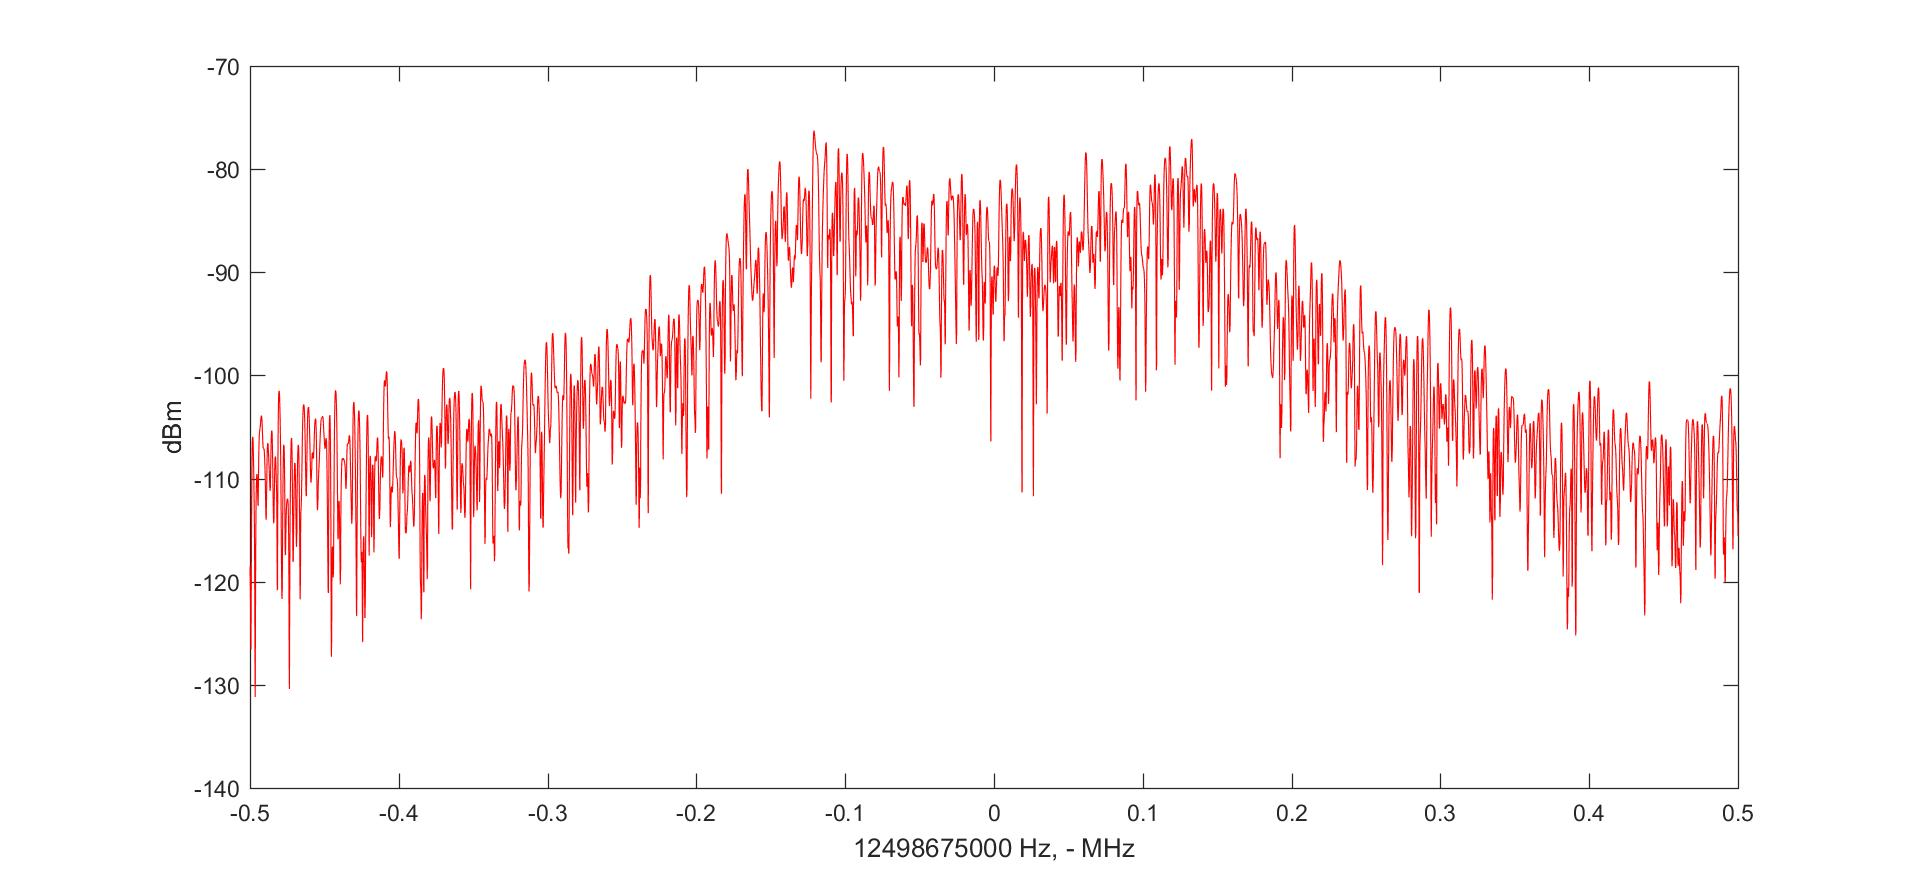
\includegraphics[width=1\linewidth]{noisy12_beatnote}
  \end{minipage}
  \caption{Слева оптический спектр оптической гребенки в шумном режиме. Справа соответствующий сигнал биений на частоте ОСД 12.48 ГГц.}
  \label{noisy12}
\end{figure}

Конический профиль растянутого волокна позволяет удобно изменять связь с модами резонатора путем его перемещения вверх, вниз и вдоль выступа резонатора и достигать оптимального положения, при котором солитонная ступенька наиболее широкая и мощная.

Для достижения солитонного режима требуется быстрая перестройка лазера, т.ч. тепловой нагрев и сдвиг моды резонатора не привел к выходу частоты лазера накачки из области существования солитона (рис. \ref{step_schematics}). Для этого подается однократное пилообразное напряжение на пьезоконтроллер частоты лазера, т.ч. окончание быстрой перестройки частоты совпало с центром области существования солитона. Для ступенек шириной более 6 МГц при мощности накачки до 120 мВт этого метода достаточно для повторяемого достижения солитонного режима в разных резонаторах см. Рис. \ref{soliton_12GHz},\ref{clean_27GHz_single_soliton}. В ходе работы были получены солитоны только в резонаторах из материала $MgF_2$, т.к. в нем при нагреве мощным лазером накачки терморефрактивный эффект компенсирует сдвиг собственных частот, вызванный тепловым расширением (в материалах $CaF_2$,$BaF_2$ при накачке мощным лазером возникают сильные термооптические осцилляции и достижение стационарного режима оптических гребенок затруднительно). В ходе работы были получены солитоны с частотами повторений от 8.5 ГГц до 27 ГГц. В резонаторах малого диаметра тепловая нелинейность преобладает и ширина солитонных ступенек меньше 1 МГц, что требует дополнительных методов настройки.

\begin{figure}[ht]
  \begin{minipage}[ht]{0.49\linewidth}\centering
    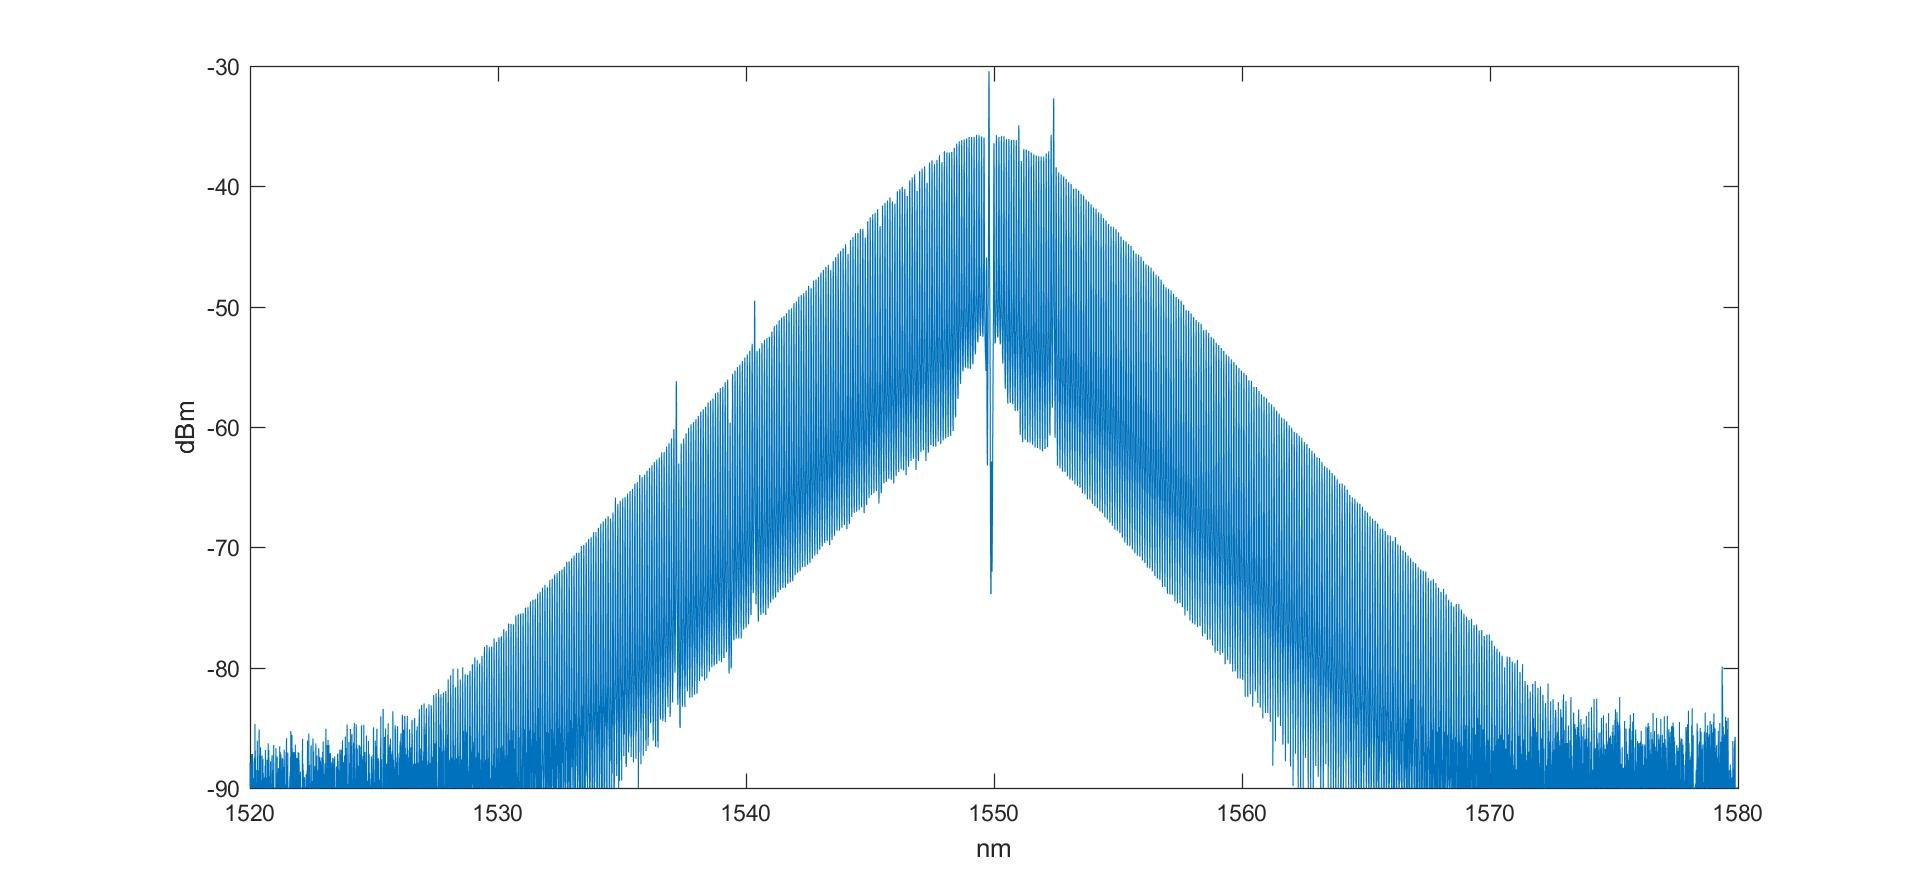
\includegraphics[width=1\linewidth]{soliton_12GHz}
  \end{minipage}
  \hfill
  \begin{minipage}[ht]{0.49\linewidth}\centering
    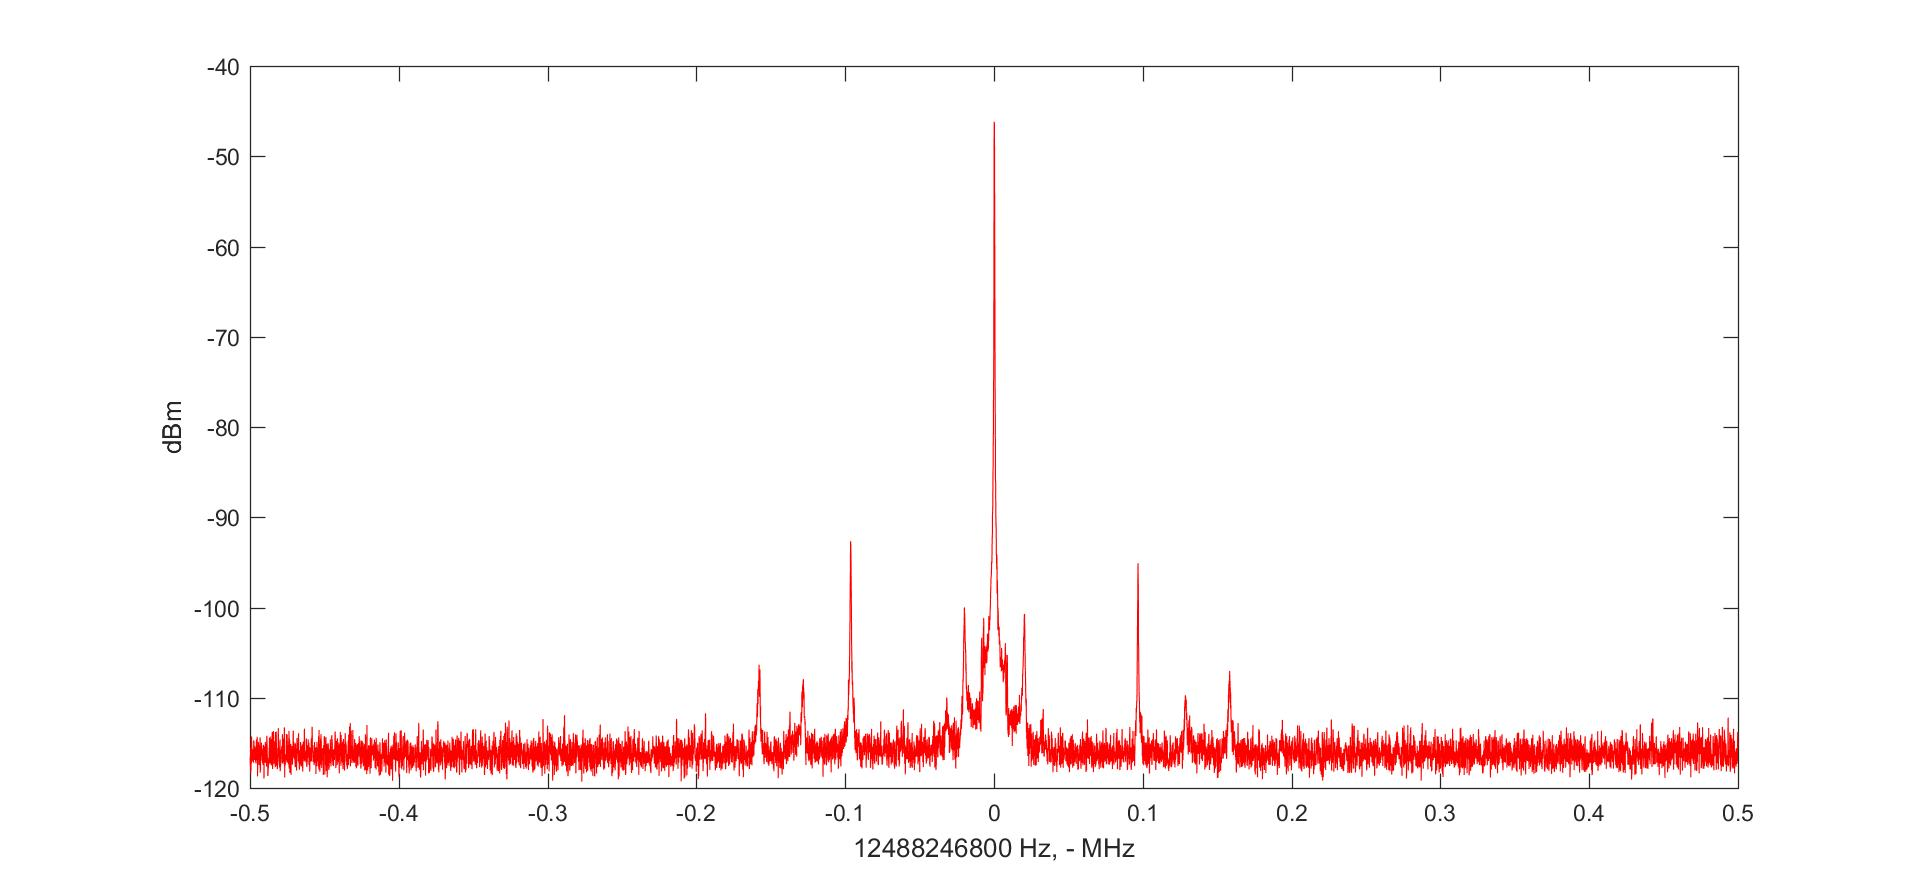
\includegraphics[width=1\linewidth]{soliton12_beatnote}
  \end{minipage}
  \caption{Слева оптический спектр оптической гребенки в односолитонном режиме. Справа соответствующий узкий сигнал биений на частоте повторения солитона 12.48 ГГц}
  \label{soliton_12GHz}
\end{figure}


\begin{figure}[ht]
  \begin{minipage}[ht]{0.49\linewidth}\centering
    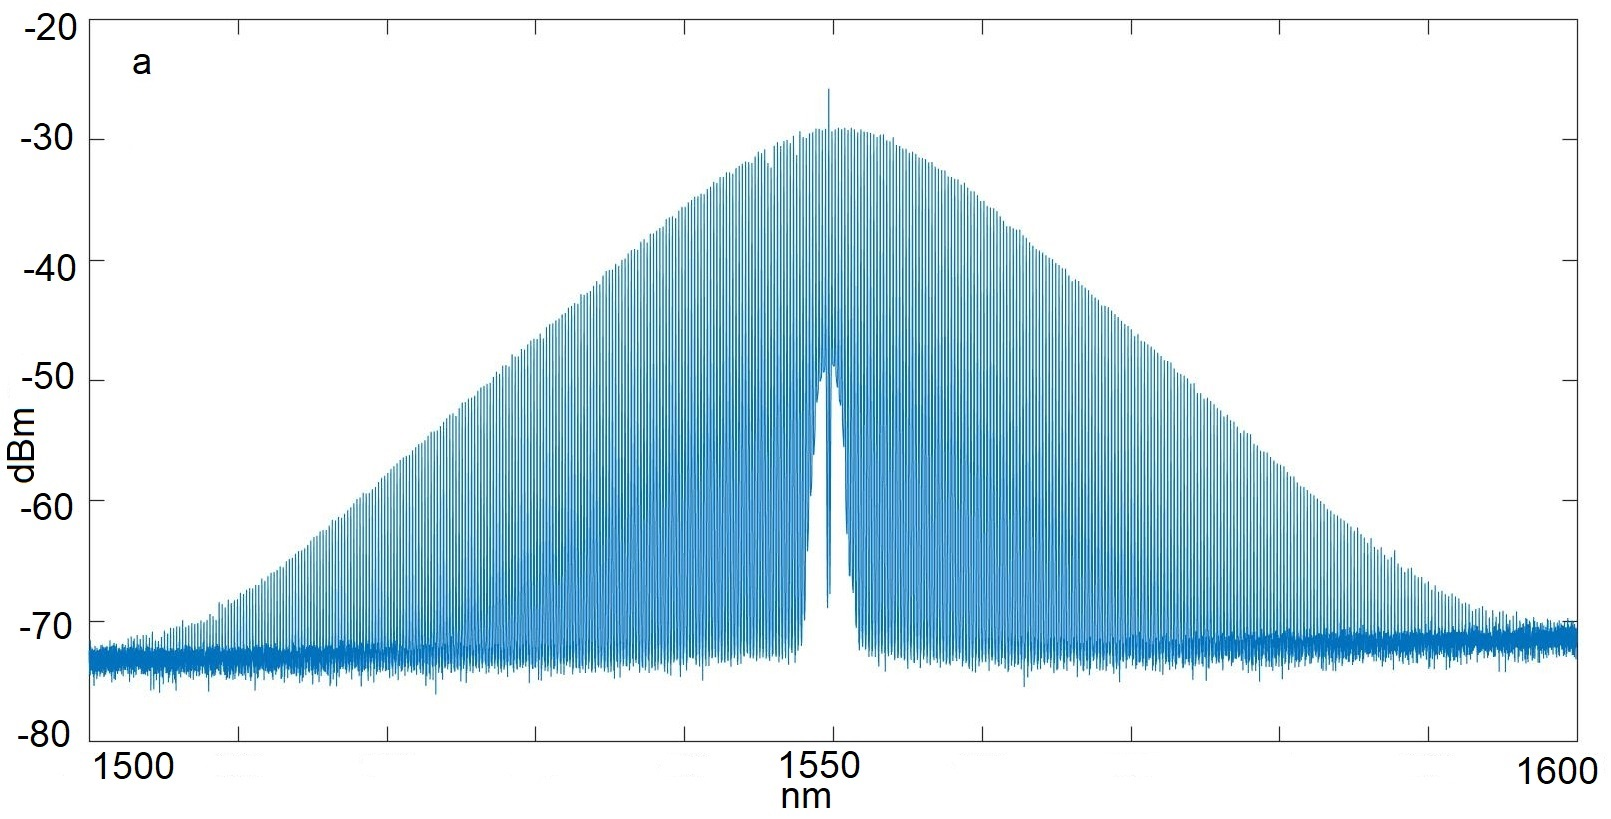
\includegraphics[width=1\linewidth]{clean_27GHz_single_soliton}
  \end{minipage}
  \hfill
  \begin{minipage}[ht]{0.49\linewidth}\centering
    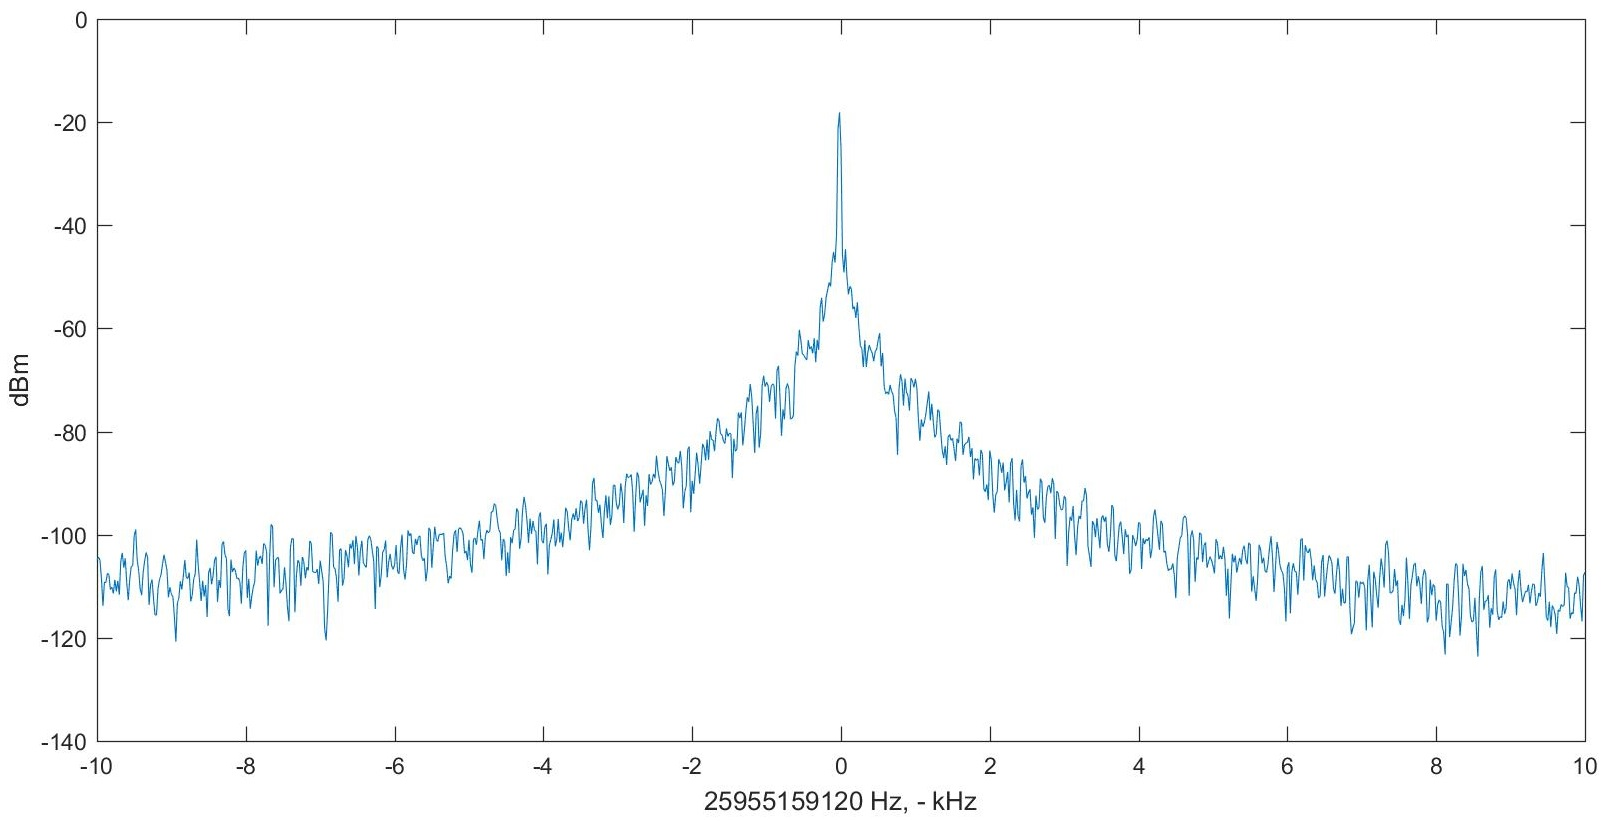
\includegraphics[width=1\linewidth]{26G_soliton_beat2}
  \end{minipage}
  \caption{Слева: Оптический спектр односолитонного режима с ОСД около 26 ГГц, полученный в резонаторе диаметром 2.4 мм и радиусом кривизны 80 мкм. Регулируя положение элемента связи (оптического волокна) с резонатором возможно добиться спектра с минимальным количеством пересечений мод и Справа: узким сигналом биений на частоте повторения солитона }
  \label{clean_27GHz_single_soliton}
\end{figure}


\begin{figure}[ht]
\centering
  
  
\end{figure}

Для контроля текущего значения отстройки лазера от частоты холодного резонанса лазер накачки фазово модулировался сигналом, подающимся с панорамного индикатора (RIGOL Network Analyser), далее сигнал пропускания системы с фотодетектора подавался на панораму и наблюдались 2 пика \ref{vna_trace}, правый пик соответствовал текущей отстройке лазера от резонанса МШГ, другой пик, на постоянной частоте, говорил о наличии солитонного режима и количестве солитонов в резонаторе \cite{Karpov2017}. Таким образом можно вручную подстраивать частоту лазера для стабилизации солитона в текущем многосолитонном и односолитонном режиме. Этот метод удобен для изучения свойств солитонов в зависимости от текущей отстройки частоты лазера, однако он неудобен для долговременной стабилизации солитонного состояния. В большинстве экспериментов с кристаллическими микрорезонаторами ширина солитонной ступеньки была не более 5 МГц (из-за относительно малой мощности накачки и потерь в растянутом волокне), и ручная настройка была затруднительна, т.к. остывание резонатора в объеме моды быстро уводило частоту лазера из области существования солитона, поэтому метод контроля отстройки с помощью фазовой модуляции накачки со сканирующей частотой не применялся.

\begin{figure}[ht]
\centering
  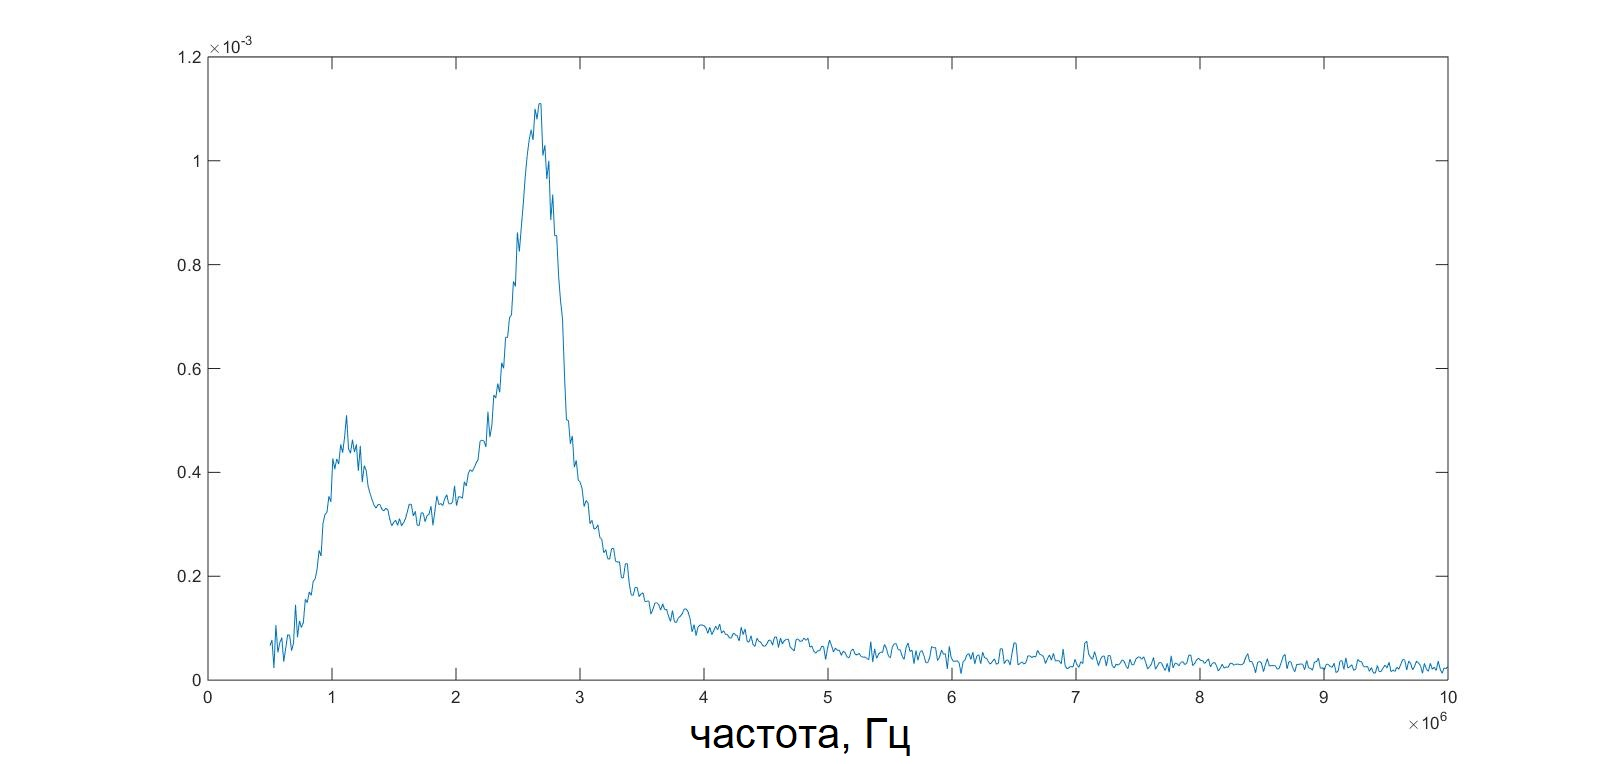
\includegraphics[width=0.5\linewidth]{vna_trace}
  \caption{Отклик системы на анализаторе цепей (панораме) при сканировании частоты фазовой модуляции. Левый пик говорит о солитонном режиме, правый показывает текущую отстройку лазера накачки от моды резонатора.}
  \label{vna_trace}
\end{figure}


Без активной стабилизации частоты лазера время жизни солитона составляло от секунды до 20 мин, за это время лазер накачки уходил из области существования солитона. Для долгосрочной стабилизации была использована схема PDH (Паунда-Древера-Холла), в котором на лазер накачки подавалась фазовая модуляция на заданной частоте, отклик системы в форме сигнала пропускания подавался на фазовой детектор вместе с исходным сигналом модуляции, сдвинуты по фазе. Получившийся сигнал ошибки подавался на PID контроллер, усиливался и подавался на пьезоконтроллер частоты лазера. Подбирая точку стабилизации на солитонной ступеньке путем изменения частоты модуляции и фазы опорного сигнала для фазового детектора, можно получить уединенный крутой склон в сигнале ошибке. Далее эмпирически подбирая параметры усиления PID контроллера, можно существенно облегчить процесс настройки на солитон - так при включенной системе обратной связи настройка на солитон путем быстрой перестройки частоты лазера дает положительный результат почти всегда. После настройки на солитонный режим включается интегратор PID на полный диапазон частот, и солитон стабилизируется на несколько часов. Недостатком схемы PDH для данной задачи является отсутствие возможности перестраивать отстройку без выключения солитонного режима. Также использовалась схема активной стабилизации температуры резонатора с помощью элемента Пельтье, диодного сенсора температуры и PID контроллера.

%\subsection{Метод стабилизации частоты повторения солитонов с помощью амплитудной модуляции лазера накачки}
%амплитудная модуляция на кратных фср частотах приводит к узкой области захватывания частоты повторения солитонов

Важным другим методом является генерация солитона при затягивании частоты лазера. В \cite{Pavlov2018} была впервые продемонстрирована возможность генерации солитонной гребенки при накачке кристаллического микрорезонатора с помощью простого лазерного диода типа Фабри-Перо. При этом продольно-многомодовый лазер, имеющий широкий дискретный спектр и большую суммарную мощность, сначала переходит в режим излучения на одной линии благодаря эффекту затягивания на высокодобротную моду микрорезонатора, с подавлением всех остальных линий в спектре в соответствии с эффектом Богатова, далее эта результирующая мощная линия является накачкой для генерации солитона в микрорезонаторе. Таким образом высокодобротный микрорезонатор одновременно выступал в роли внешнего резонатора для стабилизации лазера и в роли нелинейной среды для генерации солитонов. Методом настройки на солитонный режим была простая ручная подстройка тока на диоде, что приводило к затягиванию линии лазера, ближайшей по частоте к высокодобротной моде микрорезонатора. В эксперименте ОСД лазерного диода (17 ГГц) не совпадал и не был кратен ОСД микрорезонатора (12.1 ГГц). Используемый микрорезонатор был существенно многомодовым и содержал большое количество высокодобротных мод. Мною было экспериментально проверено, что при использовании схемы с растянутым волокном и перестраиваемым узкополосным мощным лазером накачки, наиболее мощный солитон с самой большой областью существования по отстройке, совпадал с хорошей точностью с солитоном, полученным в другом эксперименте при затягивании многочастотного лазера, в части наличия сильных эффектов нормального расщепления мод. Так дисперсия резонатора не зависит от накачки и метода связи, можно утверждать, что солитон был возбужден обоими методами на одном и том же семействе мод. Практическим недостатком метода затягивания является невозможность контролировать, какая именно мода лазера будет затянута и на какую моду микрорезонатора, поэтому повторяемо и детерминировано генерировать солитон сложно.


\subsection{Методы достижения односолитонного режима}

В литературе было предложено несколько методов детерминированного достижения односолитонного режима в оптических микрорезонаторах. Первый метод предполагает одновременную перестройку частоты лазера накачки и изменение его мощности для избежания хаотического режима гребенки \cite{Jaramillo2015}. Другим способом является не перестройка частоты лазера, а сдвиг частоты резонанса МШГ путем изменения его температуры \cite{Joshi2016} или контроля времени жизни свободных носителей (для интегральных резонаторов) \cite{Yu2016}.

Рассмотрим случай \cite{Lobanov2016} фазовой $f(t)=F e^{i\varepsilon\sin\Omega t}$ и амплитудной $f(t)=F(1+\varepsilon\cos\Omega t)$  модуляции с частотой $\Omega$ и глубиной модуляции $\varepsilon$. Моделировалась система нелинейных связанных уравнений \ref{set_am}. Тепловые эффекты не рассматривались. В численных симуляциях не рассматривались частотная зависимость нелинейности, потерь и пересечения мод, взаимодействия между модами. Предполагая, что частота модуляции близка к ОСД резонатора:

\begin{equation}
\frac{\partial a_\mu}{\partial \tau}=-(1+\zeta_\mu)a_\mu+i\sum_{\mu',\mu^{''}}a_{\mu^{'}} a_{\mu^{''}} a^{*}_{\mu^{'}+\mu^{''}-\mu}+f_{\mu}\exp(i\mu\Delta\tau).
\end{equation}

Все обозначения соответствуют принятым в этой работе для фазовой модуляции $f_\mu=F J_\mu(\varepsilon)$, для амплитудной - $f_{k}=F[\varepsilon/2,1,\varepsilon/2]$,  $f_{\mu \neq k}=0, k={-1,0,1}$, безразмерной величине накачки $F$. $J_\mu(\varepsilon)$ функция Бесселя порядка $\mu$, $\Delta=2(D_1-\Omega)/\kappa$ нормализованная отстройка от точного значения ОСД, $D_1$ соответствует $2\pi\times$FSR. Все номера мод $\mu$ определены относительно 0 моды накачки. Дисперсионный закон дается разложением $\omega_\mu=\omega_0+D_1\mu+\frac{1}{2}D_2\mu^2+...$ и пренебрегая дисперсией третьего и более высоких порядков, получаем выражение для нормализованной отстройки: $\zeta_\mu=2(\omega_0-\omega_p)/\kappa+(D_2/\kappa)\mu^2$. $D_2>0$ соответствует аномальной дисперсии. Моделировалось 525 мод. Для анализа вычислялась средняя мощность внутри резонатора $U=\sum_{\mu} \vert a_\mu\vert^2$ для разных занчений нормализованной отстройки $\zeta_0$ и соответствующий профиль поля в микрорезонаторе $\psi(\varphi)=\sum_{\mu} a_{\mu}\exp(i\mu\varphi)$.

Для возбуждения солитонов лазер накачки перестраивается линейно по частоте $\zeta_{0}(\tau)=\zeta_{0}(0)+\alpha\tau$ от эффективной синей отстройки $\zeta_0(0)<0$, через нулевую отстройку в эффективную красную область $\zeta_0\gg0$ для сканирования всей области существования солитона. Формирование солитонов дает характерные ступеньки в генерируемом свете. Если перестройку лазера остановить на частоте, лежащей на ступеньке, то солитонное состояние является стабильным во времени. Максимальная частота отстройки области существования солитона \cite{Herr2014} дается $\zeta_{0\text{max}}\sim {\pi^2 F^2}/{8}$. В симуляциях использовались следующие значения $F\approx 4.11$, $D_{2}/\kappa\approx {0.01}$ и $\zeta_{0\text{max}}\approx 20.8$

Для набора статистики проводилось по 100 симуляций для каждого набора параметров и строилось распределение вероятности количества генерируемых солитонов. Известно \cite{Herr2014, Karpov2016}, что в случае немодулированной накачки ($\varepsilon=0$) количество возбуждаемых солитонов может варьироваться от скана к скану. Это подтверждается и при численном моделировании рис. \ref{Mod4}(a)-\ref{Mod4}(b). Среднее количество возбуждаемых солитонов увеличивается с увеличением мощности накачки и уменьшении ДГС резонатора. При уменьшении скорости сканирования лазера более вероятными становятся малосолитонные режимы.

\begin{figure}[ht]
\centering
  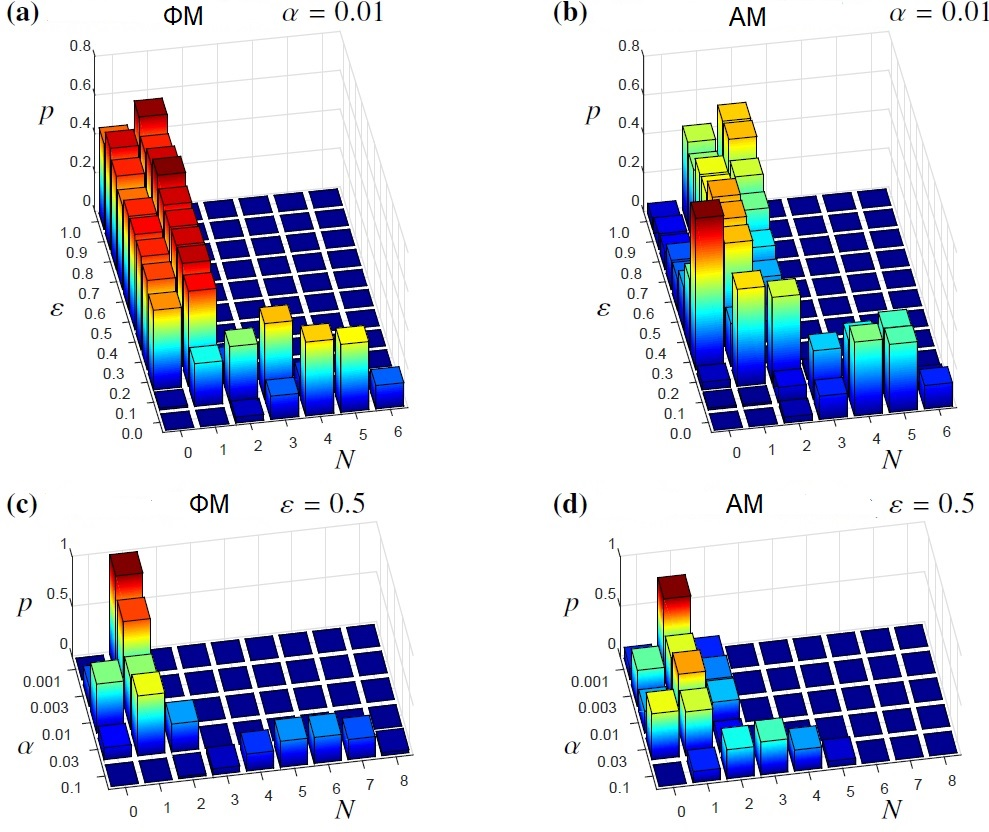
\includegraphics[width=0.85\linewidth]{Modulation4_s}
  \caption{Распределение вероятностей количества возбужденных солитонов от глубины модуляции $\varepsilon$ и скорости сканирования $\alpha$. Конечная отстройка $\zeta_0=18$ для фазовой и $\zeta_0=15$ для амплитудной модуляции. В обоих случаях $F\approx 4.11$, $100$ реализаций.}
  \label{Mod4}
\end{figure}

Статистика значительно изменяется при включении слабой резонансной модуляции ($\Delta=0$) на частоте строго равной 1 ОСД резонатора. Как только глубина модуляции достаточно высокая ($\varepsilon> 0.2$), то более вероятными становятся состояния с меньшим количеством солитонов (см рис. \ref{Mod4}(a)-\ref{Mod4}(b)). Для фазовой модуляции возможны два равновероятных сценария - возбуждение односолитонного режима или отсутствие генерации солитонов вообще. Для амлитудной модуляции наиболее вероятные сценарии одно- или двухсолитонные состояния. Этот факт может быть объяснен взаимодействием солитонов: под действием фазовой модуляции солитоны внутри микрорезонатора двигаются к положению равновесия. Два солитона сталкиваются и уничтожаются, т.ч. суммарное число солитонов уменьшается на 2. Либо два солиотна сливаются в один с уменьшением общего числа на 1.

Важным фактором увеличивающем вероятность односолитонного режима является уменьшение скорости сканирования частоты лазера. При малых $\alpha$ для детерминированного достижения односолитонного режима требуется меньшая глубина модуляции. После остановки перестройки частоты лазера и достижения солитонного режима, возможно отключение модуляции с сохранением солитона, если глубина модуляции невелика.

При модуляции не строго на частоте 1 ОСД, а с неточностью $\Delta$, вероятность достижения односолитонного режима ниже и предложенный метод не так эффективен, что частично можно компенсировать увеличением глубины модуляции.

%\begin{figure}[ht]
%\centering
%  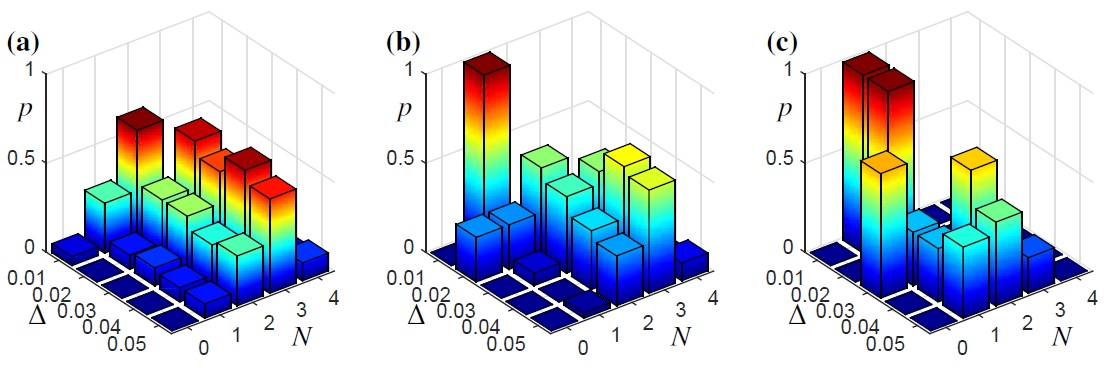
\includegraphics[width=0.85\linewidth]{detuned}
%  \caption{Распределение вероятностей количества возбужденных солитонов при фазовой модуляции для различных значений неточности $ \Delta$  и $\varepsilon$  при  $\alpha=0.001$, $\frac{D_2}{\kappa}\approx 0.01 $. Конечная отстройка $\zeta_0=18$: (a) $\varepsilon=0.3$; (b) $\varepsilon=0.6$; (c) $\varepsilon=1.0$.}
%  \label{Detuned}
%\end{figure}

Для подтверждения численных симуляций был проведен эксперимент с резонатором из $MgF_2$. Резонатор имел диаметр 5.6 мм, радиус кривизны 35 мкм. Нагруженная ширина линии составила 500 кГц. Экспериментальная установка представлена на рис. \ref{chaos_order_experiment}(a) и полностью аналогична стандартной схеме.

\begin{figure}[ht]
\centering
  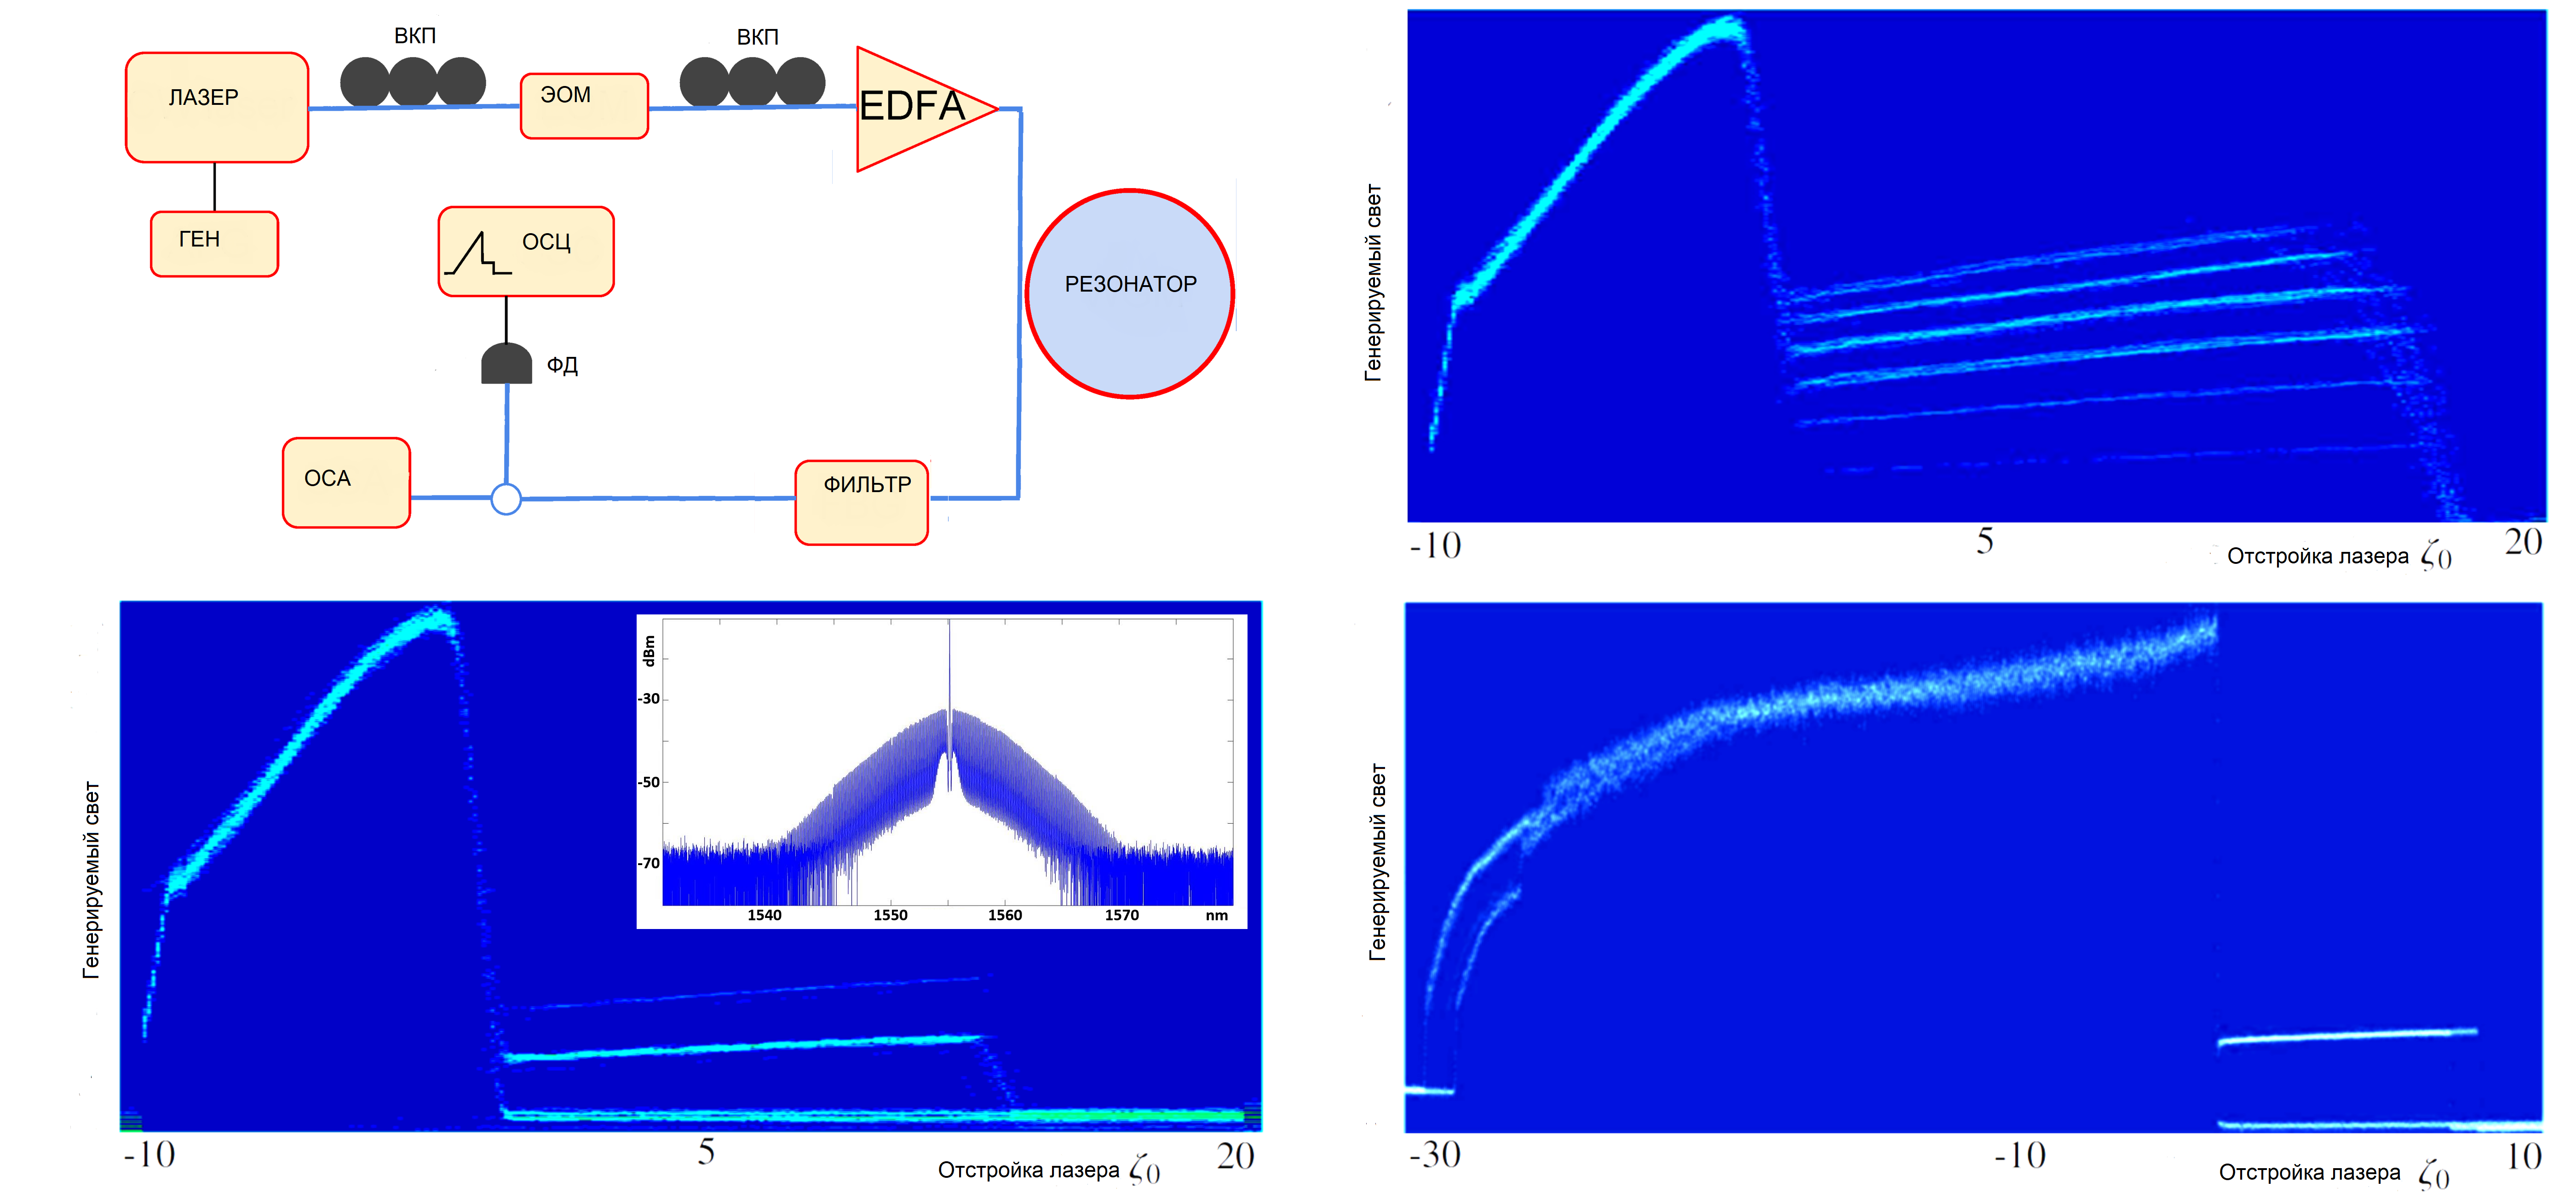
\includegraphics[width=1\linewidth]{Experiment_s}
  \caption{Экспериментальное измерение формирования солитонов при фазовой модуляции накачки и сканировании лазера. (a) экспериментальная установка (AFG, генератор сигналов произвольной формы; CW laser, узкополосный перестраиваемый лазер непрерывной мощности; FPC, волоконный контроллер поляризации, EDFA, эрбиевый волоконный усилитель; WGM,  микрорезонатор из MgF$_2$; FBG, волоконный Брэгговский фильтр; PD, фотодиод; OSA, оптический спектроанализатор; OSC, осциллограф); (b) статистика 100 измерений по осциллографу сканирования лазера нелинейной моды резонатора на частоте 100 Гц, показана зависимость генерируемого света от отстройки частоты лазера без внешней модуляции, (c) статистика при включенной фазовой модуляции, частота сканирования лазера 100 Гц, вероятность отсутствия солитонов - 0.5, генерации 1 солитона - 0.4, двух солитонов - 0.1, вставка показывает оптический спектр односолитонного режима с $\text{sech}^2(x)$ огибающей, ширина спектра 35 нм, расстояние между линиями соответствует 1 ОСД резонатора в 12.1 ГГц; (d) статистика 100 измерений при включенной амплитудной модуляции, частота сканирования лазера 5 Гц, вероятность отсутствия солитонов - 0.4, генерации 1 солитона - 0.6.}
  \label{chaos_order_experiment}
\end{figure}

Накачивая резонатор лазером мощностью 100 мВт после усилителя на длине волны 1554 нм наблюдаются характерные ступеньки в сигнале генерируемого света, соответствующие формированию солитонов. Оптический спектр односолитонного режима приведен на вставке рис. \ref{chaos_order_experiment}(c).

Экспериментально были проверены разные разные скорости сканирования частоты лазера от 0.25 ГГц/с до 25 ГГц/с ($\alpha \approx 0.0006...0.06$). Одновременно была приложена либо фазовая либо амплитудная модуляция накачки с помощью волоконного электрооптического модулятора. Глубина амплитудной и фазовой модуляции была около -26 дБн ($\varepsilon \approx 0.1$). Для анализа были записаны по 100 сигналов с фотодектора для каждого набора параметров.

Рис. \ref{chaos_order_experiment}(b)-\ref{chaos_order_experiment}(d) показывает наложенные друг на друга данные от 100 измерений, демонстрируя статистику генерации солитонов, т.ч. более яркие кривые означают более высокую вероятность такого сценария. Было обнаружено, что оптимальная частота модуляции, при которой наблюдался наиболее вероятный односолитонный режим была близка, но не совпадала точно с частотой $12.1025$ ГГц - ОСД "горячего" резонатора, который был измерен по сигналу биений в солитонном режиме. Оптимальное отличие частоты модуляции от этого значения ОСД составило около 1 МГц (что значительно больше суммарной дисперсии резонатора). При этом отклонение частоты от оптимальной более, чем на 100 кГц приводило к исчезновению эффекта более вероятной односолитонной генерации. Такое отклонение оптимально частоты от ОСД может быть объяснено тем, что ОСД холодного резонатора из численной модели отличается от измеренного ОСД нагретого резонатора в эксперименте. Из экспериментальных данных видно, как фазовая так и амплитудная модуляция накачки радикально меняется распределение вероятностей для числа генерируемых солитонов, т.ч. односолитонный режим становится достижимым и наиболее вероятным. Хотя эксперимент хорошо качественно согласуется с численным моделированием, видны отличия из-за неучтенных эффектов, вызванных дисперсией более высокого порядка и тепловыми эффектами.

\subsection{Исследование зависимости свойств солитонов от отстройки частоты лазера накачки}

Ключевым параметром, описывающим динамику частотных гребенок и солитонов в микрорезонаторах является эффективная отстройка частоты лазера накачки от частоты резонанса под действием тепловой и керровской нелинейности. Рассматривая приближенное решение стационарного уравнения Луджиато-Лефевера без члена, отвечающего за диссипацию, \ref{initial_cond_soliton} получаем после Фурье преобразования к спектральному представлению $\Psi(\mu)=\sqrt{d_2/2} sech(\frac{\pi\mu}{2}\sqrt{d_2/\zeta_o})$ или, выражая через оптическую частоту: $\Psi(\omega-\omega_p)=\sqrt{d_2/2} sech(\frac{\omega-\omega_p}{\delta\omega}), \delta\omega=\frac{2D_1}{\pi}\sqrt{\frac{\zeta_0}{d_2}}$, откуда видно что ширина гребенка пропорциональна квадратному корню из отстройки. Тем самым можно варьировать мощность солитона и его длительность. При увеличении отстройки лазера мощность солитона растет, а длительность уменьшается \ref{detuning_dependant}. Область существования солитона по отстройке определяется из условий существования действительных корней в стационарном уравнении на $\psi_0$ для минимальной отстройки, а максимальная отстройка берется из условий существования решений на фазу солитона: $\zeta_0\geq\sqrt{3}$, $\zeta_0\leq \pi^2 f^2/8$. Также величина отстройки ограничивает максимально допустимое число солитонов в мультисолитонном режиме, которые могут распространяться без взаимодействия: $N_{max}<\frac{\pi\sqrt{\zeta_0}}{2\sqrt{2}}$. При малых отстройках численно и экспериментально, как правило, наблюдаются бризерные режимы солитонов.

Экспериментально диапазон существования солитона может быть измерен калибровкой длины солитонной ступеньки, например, с помощью фазовой модуляции лазера накачки в схеме стабилизации PDH, тогда эффективная отстройка будет соответствовать частоте модуляции (точке, в которой сигнал ошибки пересекает солитонную ступеньку). Непрерывно менять отстройку можно в схеме без стабилизации, однако необходимо отслеживать текущее значение отстройки с помощью анализатора цепей (панорамы). Все используемые кристаллические резонаторы являются существенно многомодовыми, поэтому очень часто экспериментально наблюдаются эффекты нормального расщепления мод, когда оптическая мощность эффективно перекачивается в другие семейства мод (см рис. \ref{17G_100nm_single_soliton_amx}), т.к. локально нарушается закон дисперсии и для моды из другого семейства выполняются фазовые условия синхронизма. Интенсивность спектральных пиков (дисперсионных волн) зависит от отстройки лазера накачки (не гладко, а скачкообразно), а положение определяется дисперсионными характеристиками резонатора и величиной связи с этими семействами мод. Такие интенсивные дисперсионные волны приводят к спектральному сдвигу центра солитона (максимума огибающей спектра) в противоположную от пика сторону. Сдвиг спектрального макимума солитона ($\Omega$) приводит к пропорциональному изменению частоты повторения солитона: $\delta f_{rep}=\frac{D_2\Omega}{D_1}$ \cite{Yang:16}. Экспериментально это может позволить вычислить дисперсию второго порядка при наличии заметных сдвигов центра солитона. Важно отметить, что экспериментально при использовании растянутого волокна в качестве элемента связи, связь с исследуемой модой и другими семействами может меняться от измерения к измерению из-за тепловых сдвигов тонкого волокна относительно поверхности резонатора, поэтому проследить изменение абсолютных величин мощности линий гребенки от реализаций эксперимента затруднительно. Также экспериментально многократно использовалось преимущество растянутого волокна - возможность тонко менять связь с различными семействами мод, тем сам уменьшая эффекты нормального расщепления мод. Наличие сильной перекачки мощности в другие семейства мод приводит к значительному ухудшению фазовых шумов сигнала биений на частоте повторения солитона.

\begin{figure}[ht]
\centering
  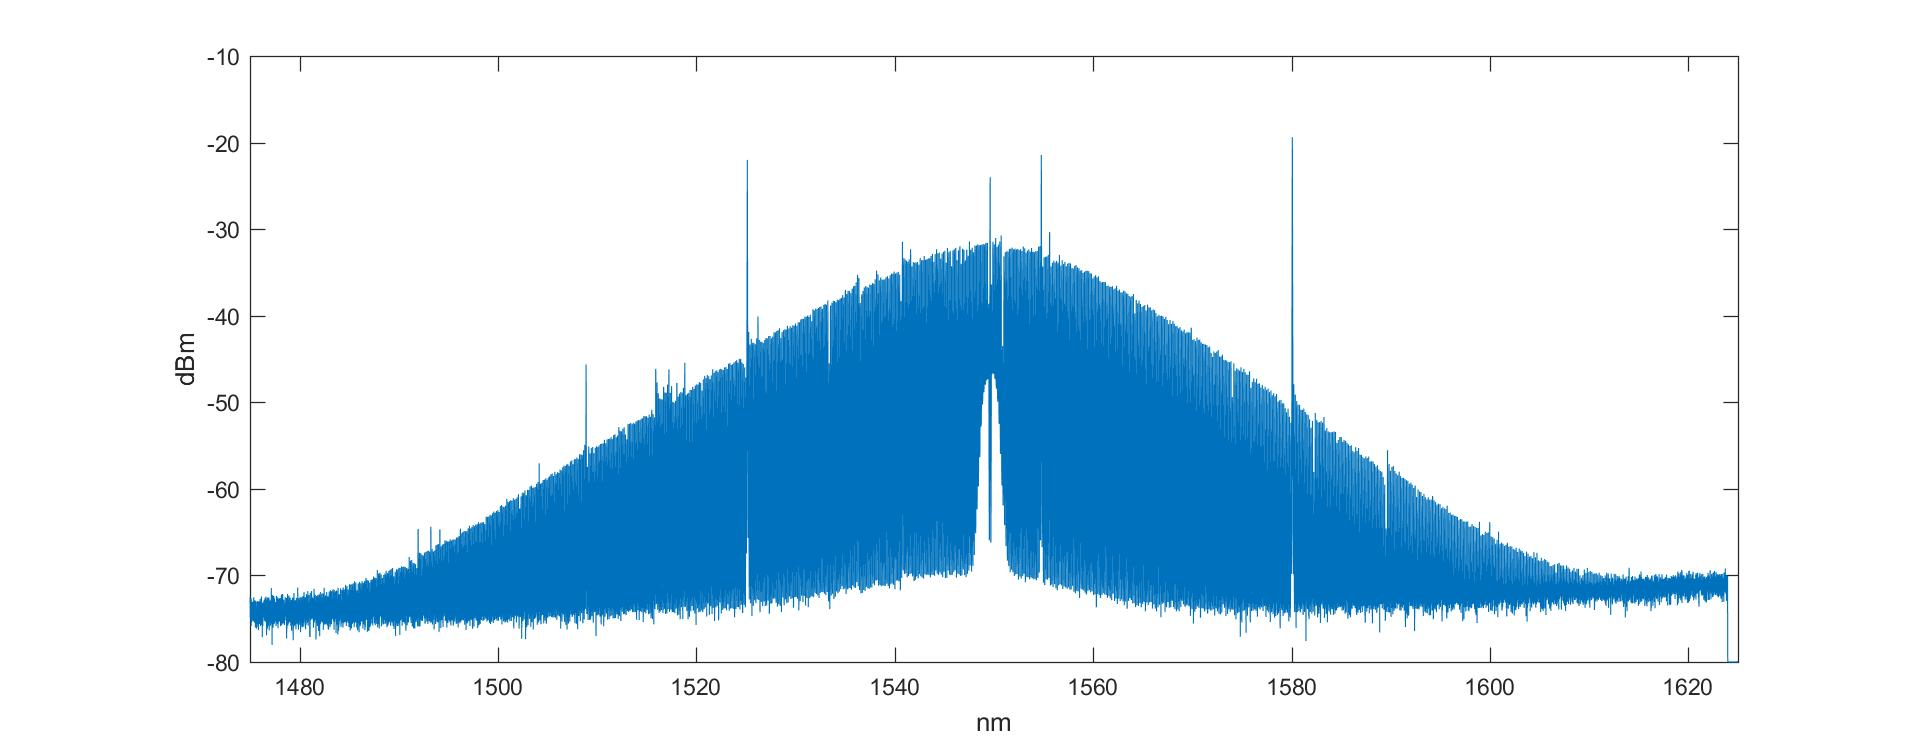
\includegraphics[width=0.5\linewidth]{17G_100nm_single_soliton}
  \caption{Оптический спектр солитона с многочисленными мощными пиками возбужденных мод из других семейств, их суммарная мощность больше, чем мощность самого солитона.}
  \label{17G_100nm_single_soliton_amx}
\end{figure}

Зависимость частоты повторения солитона от отстройки лазера, возникающая из-за наличия дисперсии высоких порядков ($D_3,D_4$), эффектов нормального расщепления мод или Рамановского рассеяния, является ключевым условием возможности наблюдения двух оптических гребенок на одном семействе мод, распространяющихся как в одном, так и в противоположных направлениях.

\subsection{Исследование метода долговременной стабилизации частоты повторения солитона}

Пример нестабильности частоты повторения солитона без стабилизации отстройки дан на рис. \ref{beatnote_drift_2min} и составляет порядка 5 кГц за 2 мин.

\begin{figure}[ht]
\centering
  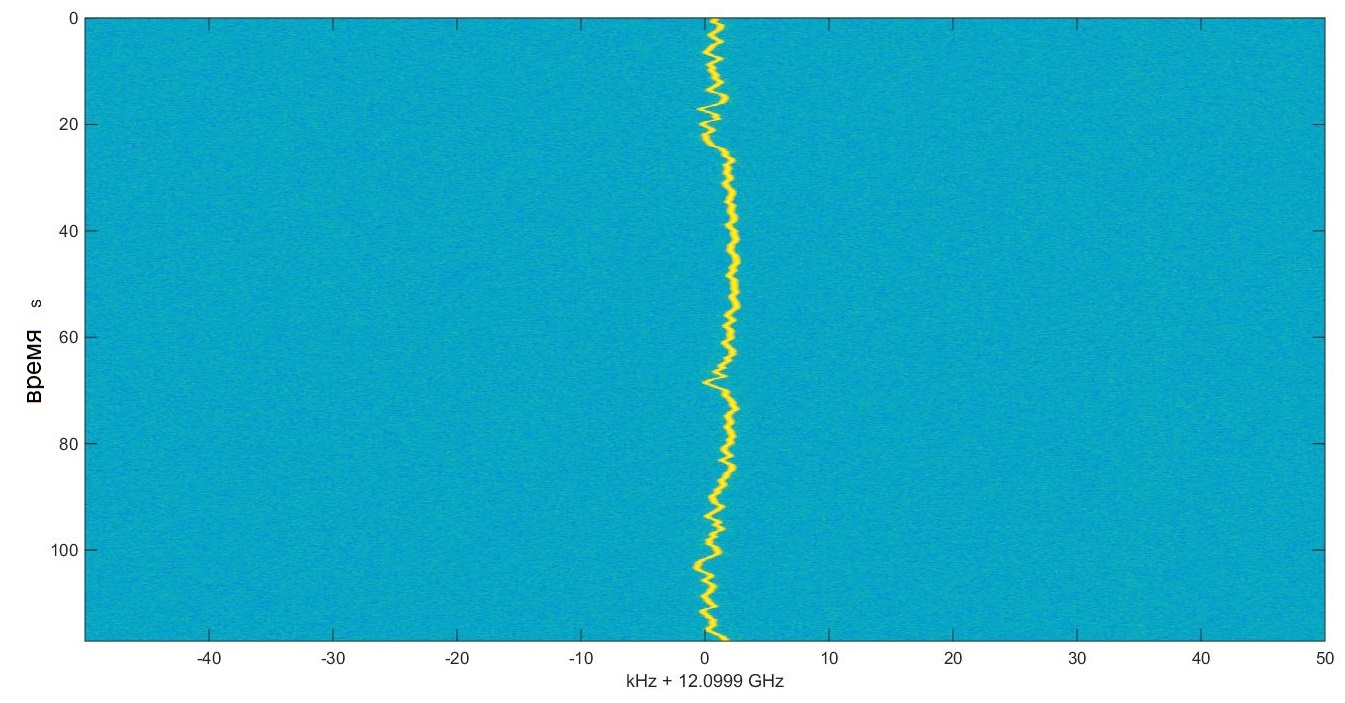
\includegraphics[width=0.5\linewidth]{beatnote_drift_2min}
  \caption{Нестабильности частоты повторения солитона без стабилизации отстройки за 2 мин порядка 5 кГц}
  \label{beatnote_drift_2min}
\end{figure}

Экспериментально в схеме \ref{Setup_CoProp} было выявлено, что при фазовой или амплитудной модуляции лазера накачки строго на частоте повторения солитона, возможно захватывание частоты биений солитона на боковую линию модуляции, т.ч. стабильность частоты повторения солитона на длинных временах определяется стабильностью задающего генератора. Однако измеренный диапазон захватывания составляет не более 1 кГц (при частоте повторения в 14.1 ГГц) \ref{rep_rate_locking}.

\begin{figure}[ht]
\centering
  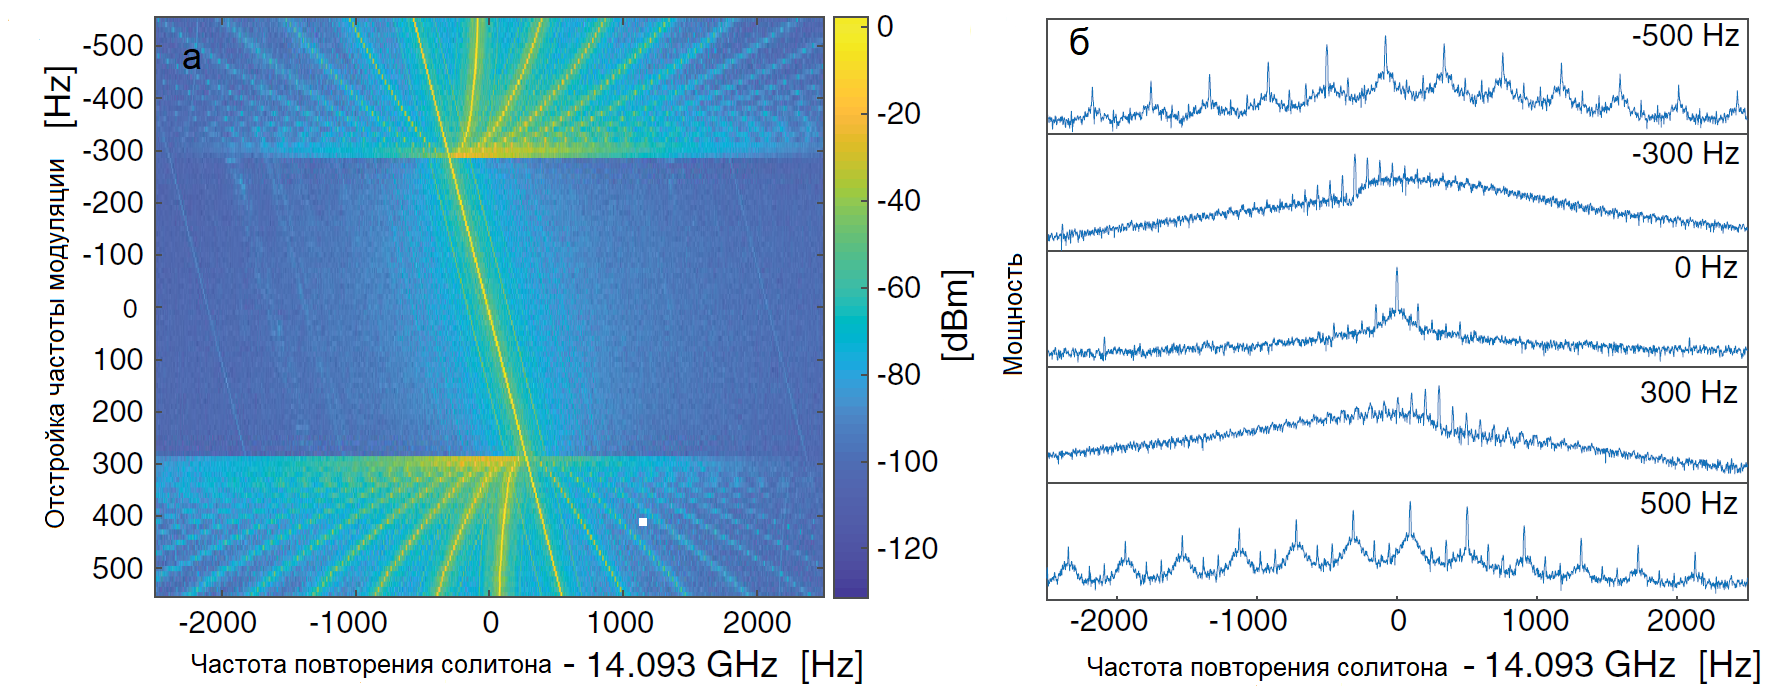
\includegraphics[width=0.8\linewidth]{rep_rate_locking}
  \caption{Слева: спектрограмма эффекта захватывания частоты повторения солитона на линейно перестраиваемую частоту фазовой модуляции лазера накачки, видна область затягивания шириной 600 Гц, Справа: спектр сигнала на быстром фотодетекторе в режиме без захватывания (-500 Гц) и с захватыванием (0 Гц).}
  \label{rep_rate_locking}
\end{figure}


\section{Экспериментальное наблюдение вынужденного комбинационного рассеяния и рассеяния Мандельштама-Бриллюэна в кристаллических микрорезонаторах}

Суммарная (материальная + геометрическая) ДГС резонатора из $BaF_2$ является нормальной на 1550 нм, поэтому генерация светлых солитонов невозможна. При исследовании резонаторов из $BaF_2$ при накачке на длине волны 1550 нм наблюдались эффекты вынужденного комбинационного рассеяния (эффект Рамана) и рассеяния Мандельштама-Бриллюэна (ВРБ).

Фторид бария имеет отрицательный терморефрактивный ($-19\times10^{-6}/C^{o}$) и положительный термоэластичный коэффициенты ($18.1\times10^{-6}/C^{o}$). При накачке большой оптической мощностью наблюдались периодические термооптические осцилляции, которые не позволяют настроить частоту лазера на моду (Рис. \ref{baf_thermoptic}). При настройке лазера на моду резонатора объем моды нагревается быстро, потом диффузией тепло распространяется в объеме всего кристаллического диска. Сдвиг частоты моды происходит из-за зависимости показателя преломления от температуры (терморефракция), а также из-за теплового расширения материала. Пусть сначала лазер строго в резонансе с модой резонатора. Объем моды быстро нагревается, температура увеличивается и резонанс сдвигается в синюю сторону (в область более высоких частот) из-за терморефракции. Лазер перестает накачивать моду, объем моды остывает, тепло распространяется по объему всего диска, он расширяется, сдвигая собственную частоту мод в красную сторону, лазер медленно начинает разогревать моду. Мода при этом выглядит как стандартная нелинейная мода с тепловой нелинейностью при сканировании частоты, далее на определенной отстройке лазер срывается с нелинейной моды. Далее объем всего резонатора начинает остывать, моды сдвигаются и через определенное время лазер заново начинает накачивать моду, но со стороны красной отстройки. Процесс периодически повторяется. Важно отметить, что при использовании электрической схемы привязки частоты лазера PDH, и плавном увеличении мощности лазер можно привязать к нелинейной моде $BaF_2$ на длительное время.

Отметим, что для связи с резонатором из $BaF_2$ при накачке на длине волны 1550 нм с показателем преломления $n=1.4661$ использовалось растянутое волокно SMF28 из плавленого кварца с $n=1.452$ для ядра волокна. В теории элемент связи должен иметь больший показатель преломления, чем материал резонатора для эффективной связи. Однако экспериментально изготовить растянутое волокно для связи с резонатором из фторидом бария оказалось даже легче, чем для связи с резонатором из фторида магния, т.к. уже при толщине волокна порядка 7-8 мкм наблюдалась связь. Также была достигнута критическая связь с растянутым волокном.

\begin{figure}[ht]
\begin{minipage}[ht]{0.49\linewidth}\centering
    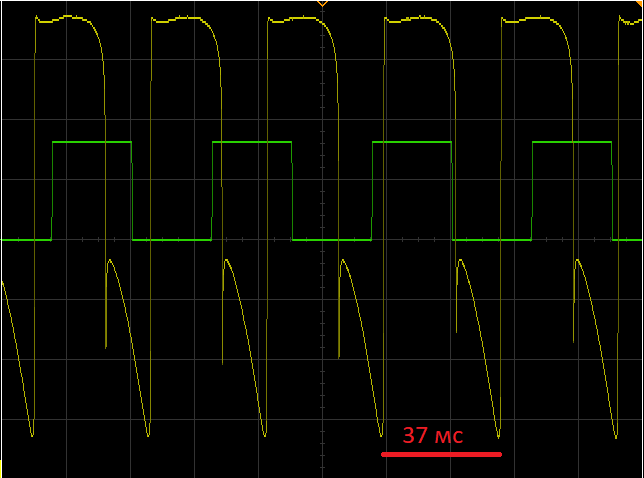
\includegraphics[width=1\linewidth]{baf_thermoptic}
  \end{minipage}
  \hfill
  \begin{minipage}[ht]{0.49\linewidth}\centering
    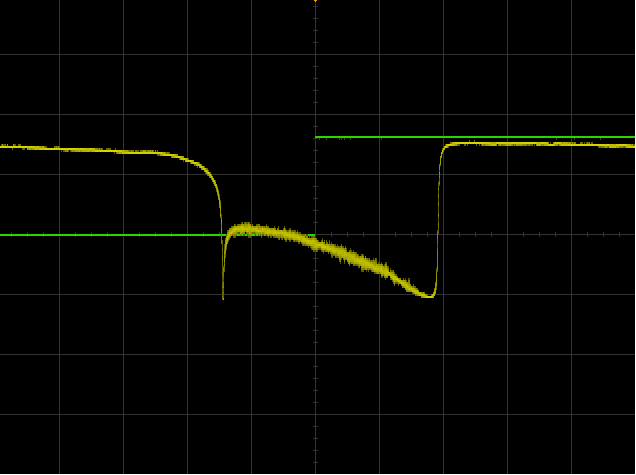
\includegraphics[width=1\linewidth]{baf_themoopticsingle}
  \end{minipage}
    \caption{Термооптические осцилляции в резонаторе $BaF_2$ диаметром 1 мм при накачке мощностью 25 мВт на 1550 нм. По оси абсцисс время, по оси ординат пропускание системы в относительных единицах.}
  \label{baf_thermoptic}
\end{figure}

При диаметре резонатора из $BaF_2$ 400 мкм, и радиусе кривизны 100 мкм (ОСД 162.7 GHz и расстояние между линиями гребенки 1.3 нм) геометрическая дисперсия уже компенсирует нормальную материальную дисперсию и суммарная дисперсия аномальная. Поэтому удалось наблюдать каскадную генерацию нескольких линий гребенки на значительном удалении от моды накачки и одновременно генерацию вынужденного рамановского излучения на длине волны 1615 нм, что соответствует табличному значению для рамановского сдвига в материале (см рис. \ref{baf_comb_anomal}).

\begin{figure}[ht]
\begin{minipage}[ht]{0.49\linewidth}\centering
    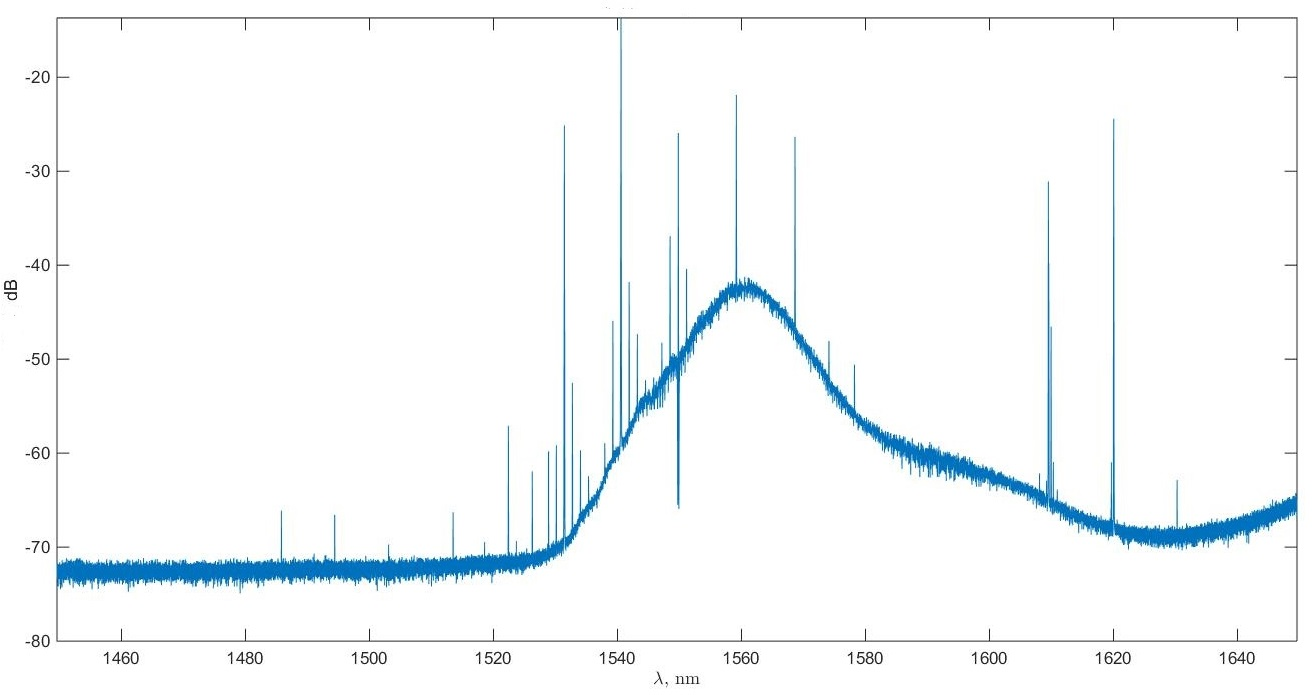
\includegraphics[width=1\linewidth]{b44_3}
  \end{minipage}
  \hfill
  \begin{minipage}[ht]{0.49\linewidth}\centering
    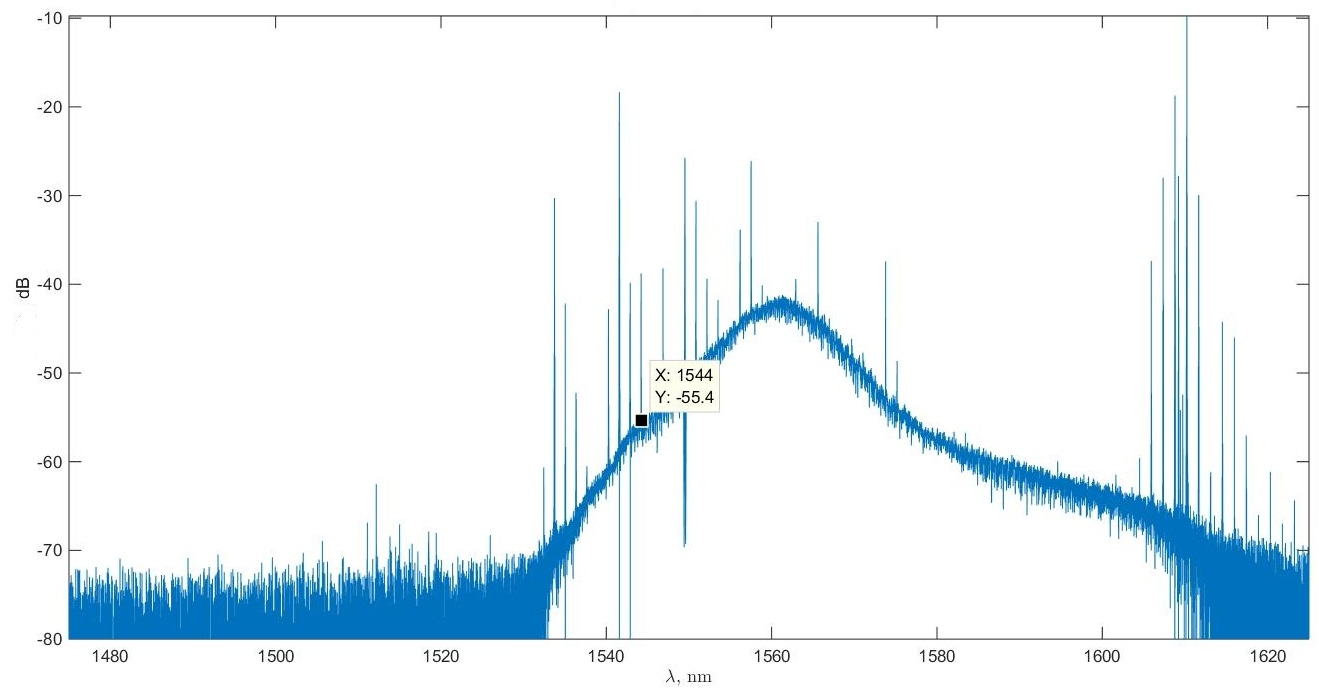
\includegraphics[width=1\linewidth]{b44_4}
  \end{minipage}
    \caption{Оптический спектр вынужденного Рамановского рассеяния и генерации оптической гребенки в резонаторе $BaF_2$ диаметром 400 мкм при аномальной дисперсии групповой скорости.}
  \label{baf_comb_anomal}
\end{figure}

В другом резонаторе из $BaF_2$ с диаметром 3.9 мм, ОСД 16.689 ГГц, с радиусом кривизны 500 мкм существенно больше семейств возбуждаемых мод, они расположены близко друг к другу и при большой мощности в нелинейном режиме перекрываются. Бриллюэновская частота сдвига не совпадает с ОСД фундаметального семейства мод (16.689 ГГц). Резонансное рассеяние света на акустических колебаниях кристаллической решетки происходит в ширине полосы Бриллюэна и усиление просходит на модах из другого семейства, чем мода накачки. Бриллюэновский сдвиг вычисляется как $\nu_b=2*n_{eff}*V_a/\lambda$, где $V_a$ вычисляется через эластичные константы и плотность материала. Для накачке на длине волны 1550 нм расчетное значение $\nu_b=8.27$ ГГц. Ширина полосы усиления достаточна мала и составляет порядка 10 МГц, поэтому необходимо иметь высокодобротную моду резонатора в этом диапазоне для усиления. В исследуемом резонаторе соответственно больше мод, чем в резонаторе значительно меньшего диаметра, на которых наблюдается вынужденное рассеяние Бриллюэна, каскадно при мощности накачки в эксперименте в 25 мВт. Порог по мощности для наблюдения первого пика ВРБ был около 8 мВт, что существенно выше, чем в работах с Бриллюэновским лазером. Это связано с сравнительно невосокой добротностью мод резонатора $1*10^8$. В эксперименте наблюдались пики каскадного ВРБ на 8.2, 16.4, 24.6 ГГц, нечетные пики в отраженной волне, четные в проходящей (см. рис. \ref{baf_sbs}). Нечетные пики измерялись в отраженной волне на выходе оптического циркулятора, поставленного до элемента связи с резонатором. Усредненная ширина биений на частоте Бриллюэновского рассеяния составила около 2 МГц, такая большая ширина объясняется тем, что лазер накачки не был привязан по частоте к моде резонатора, и фактически сбор данных происходил при усреднении за большое время, по периодическим термоосцилляциям моды резонатора.

Отдельно была предпринята попытка изготовить резонатор такого диаметра, что удвоенная частота ВРБ (16.39-16.43 ГГц измеренная в предыдущем эксперименте) совпадала с ОСД резонтора. Такой резонатор был изготовлен, однако в экспериментах с ним никакой новой динамики наблюдать не удалось.

\begin{figure}[ht]
\begin{minipage}[ht]{0.49\linewidth}\centering
    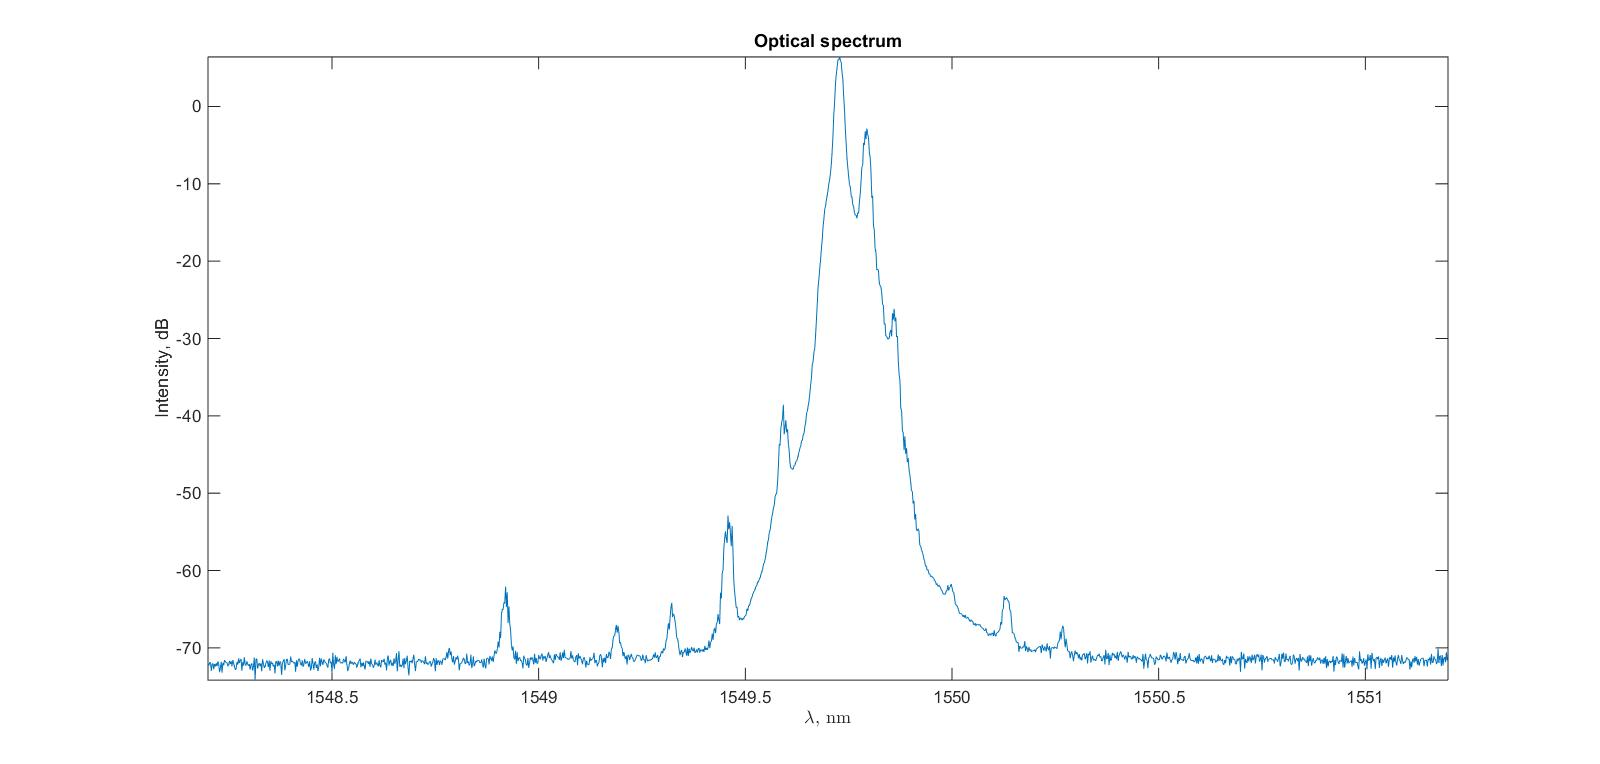
\includegraphics[width=1\linewidth]{baf_sbs_cascaded_osa}
  \end{minipage}
  \hfill
  \begin{minipage}[ht]{0.49\linewidth}\centering
    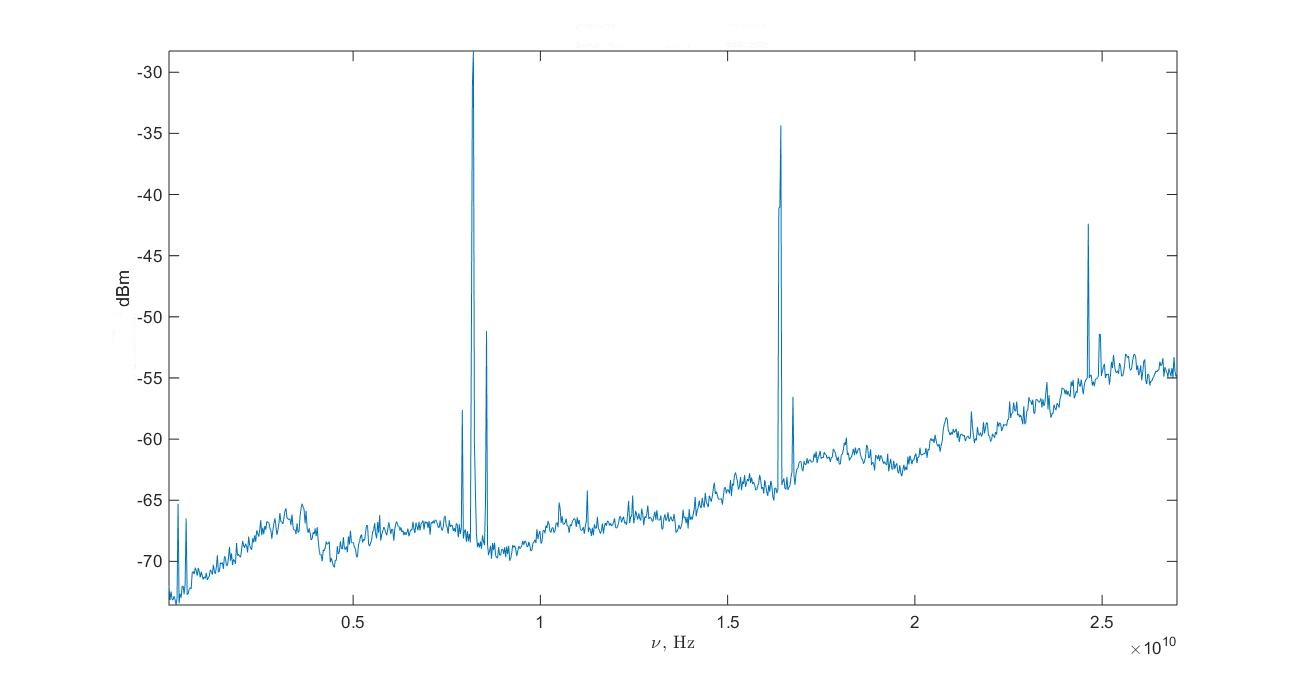
\includegraphics[width=1\linewidth]{baf_sbs_cascaded_esa}
  \end{minipage}
    \caption{Слева: оптический спектр каскадного вынужденного Бриллюэновского рассеяния (пик на 1615 нм) в резонаторе $BaF_2$ диаметром 3.9 мкм. Дисперсия резонатора нормальная, широкой керровской гребенки не наблюдалось. Справа: сигнал биений на частоте ВРБ и гармониках 8.2, 16.4, 24.6 ГГц, каждая шириной около 2 МГц.}
  \label{baf_sbs}
\end{figure}

При исследовании резонаторов из $MgF_2$ при накачке на длине волны 1300 нм, где суммарная ДГС резонатора была нормальной, была произведена попытка наблюдать генерацию оптических частотных гребенок при нормальной дисперсии с помощью двухчастотной накачки с разницей частот строго совпадающей с ОСД резонатора. Однако выходная мощность в схеме с имеющимся лазером и амплитудным электрооптическом модулятором (не волоконного, а на свободных пучках в пространстве) была недостаточна для преодоления порога по мощности. Однако впервые было наблюдено вынужденное Рамановское рассеяние в резонаторе из $MgF_2$ (см. рис. \ref{mgf_srs}), что никогда не удавалось сделать при накачке на 1550 нм при различных поляризациях. Рамановский сдвиг 410 см$^{-1}$ близок по частоте с измеренными значением 415 см$^{-1}$ для накачки на 488 нм (для группы симметрии $A_1$ тетрагональной кристаллической решетки \cite{PhysRev.154.522}). На фотодетекторе с полосой 25 ГГц наблюдался только сигнал на частоте межмодового расстояния резонатора. Два близких пика имели ширину около 200 кГц при усреднении (см. рис. \ref{mgf_srs_beatnote}). Можно предположить на основе огибающей линий в оптическом диапазоне рамановсого усиления, что возбуждались линии другого семейства, но с близкими собственными частотами. Отметим, что используемый лазер накачки имел собственную ширину линии много больше, чем ширина линии микрорезонатора, поэтому невозможно было эффективно накачать моду резонатора и стационарная картина генерации гребенки не наблюдалась, дополнительных схем стабилизации частоты не применялось.

Отдельно стоит отметить, что в многочисленных экспериментах с резонаторами из $MgF_2$ разного размера и формы, при накачке на длинах волн 1.5 и 1.65 мкм никогда не наблюдалось вынужденное рассеяние Бриллюэна ни при какой поляризации лазера накачки.

\begin{figure}[ht]
\begin{minipage}[ht]{0.49\linewidth}\centering
    \includegraphics[width=1\linewidth]{comb1330nm_raman}
  \end{minipage}
  \hfill
  \begin{minipage}[ht]{0.49\linewidth}\centering
    \includegraphics[width=1\linewidth]{comb1330nm_raman2}
  \end{minipage}
    \caption{Оптические спектры вынужденного Рамановского рассеяния (пики на 1370 нм) в резонаторе $MgF_2$ диаметром 5 мм, ОСД 12.1 ГГц, приводящие к генерации некогерентной оптической гребенки около накачки на 1300 нм, в области нормальной дисперсии резонатора. Мощность накачки 30 мВт. Слева и справа - разные накачиваемые моды.}
  \label{mgf_srs}
\end{figure}

\begin{figure}[ht]
\begin{minipage}[ht]{0.49\linewidth}\centering
    \includegraphics[width=1\linewidth]{raman_srs_zoomed}
  \end{minipage}
  \hfill
  \begin{minipage}[ht]{0.49\linewidth}\centering
    \includegraphics[width=1\linewidth]{raman_mgf_esa_beatnote}
  \end{minipage}
    \caption{Слева: Оптический спектр полосы рамановского усиления в резонаторе $MgF_2$ при накачке на 1300 нм. Справа: спектр биений на частоте межмодового расстояния резонатора 12.1 ГГц, усредненная ширина линий около 200 кГц}
  \label{mgf_srs_beatnote}
\end{figure}


%Сошлемся на все конференции \cite{confbib1,confbib2,confbib3,confbib4,confbib5,confbib6,confbib7,confbib8,confbib9,confbib10,confbib11,confbib12,confbib13,confbib14}
